\documentclass[aspectratio=169,11pt]{beamer}

% Shared style (ib-tutorials.sty at the repo root).
\makeatletter\def\input@path{{./}{../}}\makeatother
\usepackage{ib-tutorials}

\usepackage[utf8]{inputenc}
\usepackage{amsmath,amssymb}
\usepackage{booktabs}
\usepackage{array}
\newcolumntype{L}[1]{>{\raggedright\arraybackslash}p{#1}}
\usepackage{graphicx}
\graphicspath{{../pictures/4-ibfe/}{pictures/4-ibfe/}}
\usepackage{xcolor}
\usepackage{listings}
\usepackage{tikz}
\usetikzlibrary{arrows.meta,positioning,shapes.geometric,fit,calc,decorations.pathmorphing}
\usepackage{hyperref}

\newcommand{\sourcecredit}[1]{\vfill\begin{flushright}\tiny\textcolor{DarkGray}{#1}\end{flushright}}

\lstset{
  basicstyle=\ttfamily\scriptsize\color{BlackGray},
  keywordstyle=\color{NavyBlue}\bfseries,
  commentstyle=\color{DarkGray}\itshape,
  stringstyle=\color{OliveGreen},
  showstringspaces=false,
  columns=fullflexible,
  keepspaces=true,
  breaklines=true,
  breakindent=1em,
  frame=single,
  framerule=0.4pt,
  rulecolor=\color{LightGray},
  backgroundcolor=\color{LightGray!30},
  xleftmargin=0.25em,
  xrightmargin=0.25em
}
\lstdefinestyle{shell}{morecomment=[l]{\#}}
\lstdefinestyle{input}{morecomment=[l]{//}}
\lstdefinestyle{matlab}{morecomment=[l]{\%}}
\lstdefinestyle{python}{morecomment=[l]{\#}}
\lstdefinestyle{data}{}
\lstdefinestyle{tiny}{basicstyle=\ttfamily\tiny\color{BlackGray}}
\lstdefinestyle{inputtiny}{morecomment=[l]{//},basicstyle=\ttfamily\tiny\color{BlackGray}}
\lstdefinestyle{cpp}{language=C++,morecomment=[l]{//}}
\lstdefinestyle{cpptiny}{language=C++,morecomment=[l]{//},basicstyle=\ttfamily\tiny\color{BlackGray}}

\title[3D flow past objects]{3D flow past objects and the flow tank}
\subtitle{A plate across a stream in a 3D tank (IBFE/10): the gmsh volume mesh, inflow on six sides, the tether band, the initial coordinate mapping in full, the two-material plate, what a 3D run costs, the tether force as drag, and the horseshoe-crab example written up for the first time}
\author[Miller]{Laura A. Miller}
\institute[UArizona]{Department of Mathematics, University of Arizona}
\date{Using IB Software \textbullet\ Part IV \textbullet\ Chapter 22}

\begin{document}

% 1
\begin{frame}[plain]
\maketutorialtitlepanel{%
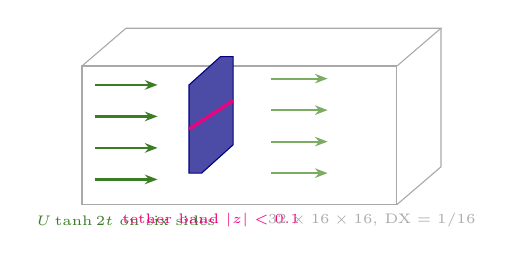
\begin{tikzpicture}[scale=0.8]
  % a box, a plate across it, stream arrows
  \draw[DarkGray,thin] (0,0) -- (5,0) -- (5,2.2) -- (0,2.2) -- cycle;
  \draw[DarkGray,thin] (0,2.2) -- (0.7,2.8) -- (5.7,2.8) -- (5,2.2);
  \draw[DarkGray,thin] (5,0) -- (5.7,0.6) -- (5.7,2.8);
  \fill[NavyBlue!70] (1.7,0.5) -- (1.9,0.5) -- (2.4,0.95) -- (2.4,2.35) -- (2.2,2.35) -- (1.7,1.9) -- cycle;
  \draw[NavyBlue] (1.7,0.5) -- (1.9,0.5) -- (2.4,0.95) -- (2.4,2.35) -- (2.2,2.35) -- (1.7,1.9) -- cycle;
  \draw[RubineRed,very thick] (1.7,1.2) -- (2.4,1.65);
  \foreach \y in {0.4,0.9,1.4,1.9} \draw[-{Stealth[length=1.6mm]},OliveGreen,thick] (0.2,\y) -- (1.2,\y);
  \foreach \y in {0.5,1.0,1.5,2.0} \draw[-{Stealth[length=1.6mm]},OliveGreen!60,thick] (3.0,\y) -- (3.9,\y);
  \node[font=\tiny,text=OliveGreen] at (0.7,-0.25) {$U\tanh 2t$ on six sides};
  \node[font=\tiny,text=RubineRed] at (2.05,-0.25) {tether band $|z| < 0.1$};
  \node[font=\tiny,text=DarkGray] at (4.6,-0.25) {$32\times16\times16$, $\mathrm{DX} = 1/16$};
\end{tikzpicture}}
\end{frame}

% 2
\begin{frame}{Learning goals}
\label{fr:goals}
\footnotesize By the end of this chapter you should be able to:
\begin{enumerate}
  \item set up a 3D flow tank: a box that is not periodic, a stream prescribed on all six faces that starts from rest, three grid levels, and a plate standing across the stream;
  \item build the plate's volume mesh in gmsh (points, lines, a surface, an extrusion, a physical volume), save it in a form libMesh reads, and know what its tetrahedra cost and where its bad elements are;
  \item write the tether band and the stress functions of IBFE/10, and use the initial coordinate mapping correctly: one mesh file, placed where you want, with the tether placed with it;
  \item give one mesh two materials by the reference position, as the 2017 version did;
  \item estimate what a 3D run costs in time and disk, run IBFE/10, read its tether force as minus the drag, and tell the force of an accelerating stream from the force of a steady one;
  \item look at a 3D run in VisIt with a slice and a displaced mesh, and describe the horseshoe-crab example, what its code measures, and what must be fixed before it is run again.
\end{enumerate}
\begin{punchbox}
\footnotesize Nothing in the IBFE code changes between 2D and 3D except \code{NDIM}; what changes is the mesh, the boundary conditions, the cost, and how you look at the result.
\end{punchbox}
\end{frame}

% 3
\begin{frame}{Where this chapter comes from}
\label{fr:sources}
\scriptsize
\begin{itemize}
  \item \al{``7-IBFE 3D Flow Tank'' (Feb 2017, edited 2018; 16 slides; the lab's weekly challenge):} goal, domain and plate dimensions, the gmsh GUI route in seven steps with screenshots, the input, ``Translate FE boundary'' with the coordinate mapping, the tether band, the two-stiffness stress functions. Its example zip \code{Example\_IBFE\_FlowTank3d-mid\_plate} (2017) is in the 2016-11 set.
  \item \al{``3-IBFE 3D Flow Past Objects'' (2020; 16 slides; \code{IBFE\_Lecture\_3}):} the same deck without the translation and the two materials (``that feature is not working as it used to in newer versions of IBAMR''), the tank moved to $-8 < x < 24$, the example named \code{3-IBFE-Example\_FlowTank-MidPlate}. Its first git version (2020-05-26) still has the removed slides; both are quoted here.
  \item \al{The 2018--20 Dogwood deck (private):} the ``3D IBFE Flow Tank'' and ``3D IBFE Free Flow'' set-ups with their numbers (tank spacing $160/256$ mm, stream $130$ mm/s), which are the horseshoe-crab example's input.
  \item \al{The horseshoe-crab example \code{3-IBFE-Example-HorseshoeCrab} (2018--2020; course repository):} a crab mesh in a free stream at $13$ cm/s, with force, velocity and work integrals. No slides were ever written for it; this chapter is the first write-up (slides \ref{fr:crab}--\ref{fr:crab4}).
  \item \al{Example IBFE/10} (this series): the course program revised, run with IBAMR 0.16.0 and 0.19.0, with the 2017 options restored as input keys and re-tested.
  \item \al{New here:} the runs and their figures; the tether force every $0.05$; the cost of the run; the coordinate mapping tested in 0.19.0 (it works); the 2017 input's tank, which was already $-8 < x < 24$ though its slides said $-16 < x < 16$; the gmsh slides' menu paths corrected; the horseshoe-crab code read and its bugs listed.
\end{itemize}
\end{frame}

% 4
\begin{frame}{Three things change in 3D}
\label{fr:three}
\footnotesize
\begin{tabular}{@{}L{0.16\textwidth}L{0.38\textwidth}L{0.38\textwidth}@{}}
\toprule
& in 2D (chapters 17--21) & in 3D (this chapter) \\
\midrule
cost & a $128\times128$ fine grid on two levels (IBFE/08), $15$ ms per step & $512\times256\times256$ fine cells if the fine level covered the tank; three levels keep it to the plate and its wake, and the run still takes $0.6$ s per step on four cores: $52$ minutes for $0.5$ time units, $3.5$ hours for the course's $2$ \\
the mesh & a \code{.mat} or \code{.msh} of triangles from MATLAB or gmsh & a volume mesh: a surface extruded into a slab, tetrahedra about $\mathrm{DX}$ across, saved as MSH 2.2; some of them flat \\
boundary conditions & periodic, or a 2D tank (chapter 7) & six faces; the stream on all of them; nothing periodic \\
looking at it & the whole field in one plot & slices, a displaced mesh, a camera (chapters 27--28) \\
the code & \code{NDIM = 2} & \code{NDIM = 3}: the same functions, \code{s(2)} and \code{X(2)} now mean something, \code{main3d} \\
\bottomrule
\end{tabular}

\medskip
The input file knows: \code{domain\_boxes} has three indices, the refinement ratios three entries, the boundary conditions six faces, and a \code{VelocityBcCoefs\_2} block exists.
\end{frame}

% 5
\begin{frame}{The set-up of IBFE/10}
\label{fr:setup}
\scriptsize
\begin{columns}[T]
\column{0.58\textwidth}
\begin{tabular}{@{}L{0.17\textwidth}L{0.78\textwidth}@{}}
\toprule
tank & $32\times16\times16$: $-8 < x < 24$, $-8 < y, z < 8$; not periodic \\
grid & $32\times16\times16$ cells on level 0 ($\mathrm{DX}_0 = 1$); three levels at ratio $4$; $\mathrm{DX} = 1/16 = 0.0625$ on the finest, which covers the plate and the flow near it \\
fluid & $\rho = 1$, $\mu = 0.01$ (\code{MU = 1/Re} with \code{Re = 100}); with the plate's width $D = 2$ and $U = 0.1$, $\rho U D/\mu = 20$ \\
stream & $(U\tanh 2t, 0, 0)$ on all six faces, $U = 0.1$: from rest to $96\%$ of $U$ by $t = 1$, $76\%$ at $t = 0.5$ \\
plate & $0.125$ thick ($0 < x < 0.125$), $2\times2$ ($-1 < y, z < 1$); \code{plate2.msh}, $3386$ nodes, $11481$ tetrahedra \\
material & compressible neo-Hookean, $\mathbb{P} = \mu_s\mathbb{F} + (-\mu_s + \beta\ln J)\mathbb{F}^{-T}$, $\mu_s = 0.538$, $\beta = 0.404$ (chapter 19) \\
tether & the band $|s_2| < 0.1$ across the middle, $\kappa_s = 10^5$, pulled to its starting position; the two flaps above and below are free \\
time & \code{DT = 1e-4}, $5000$ steps to $t = 0.5$ (the course ran to $2$); $21$ frames, $100$ force lines \\
\bottomrule
\end{tabular}
\column{0.4\textwidth}
\centering
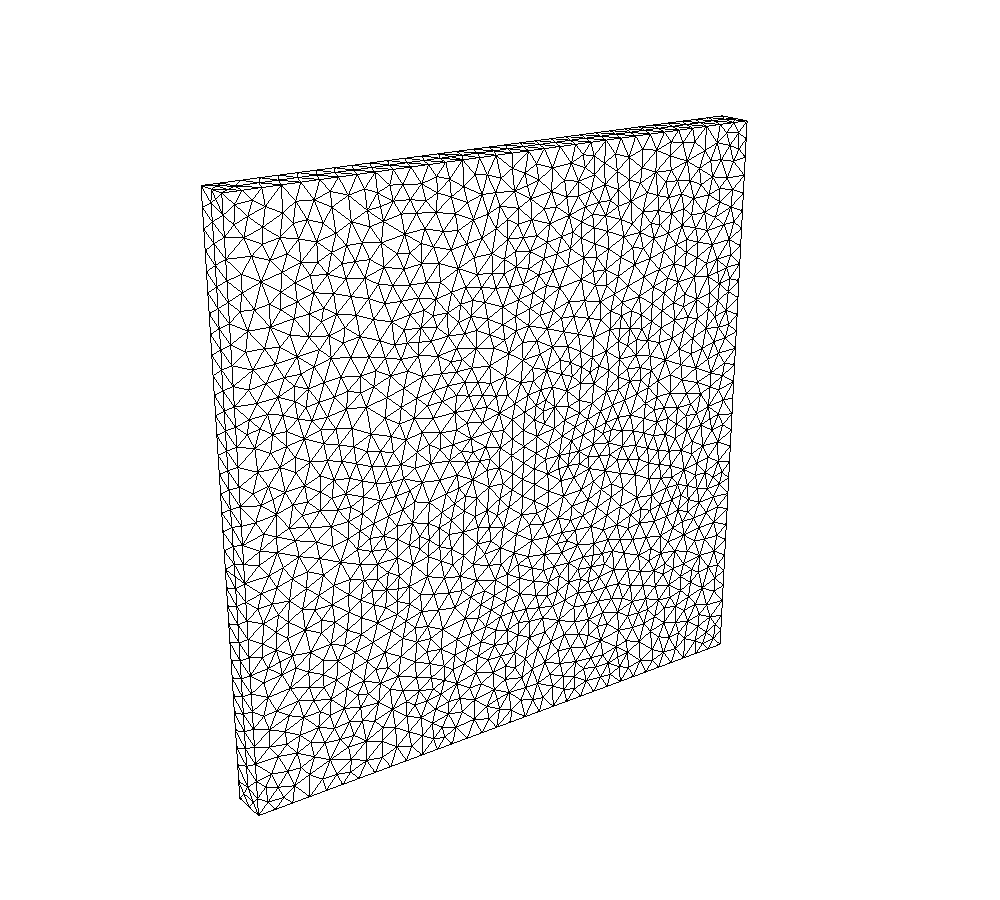
\includegraphics[width=0.8\textwidth]{ch22-plate-mesh.png}\\
The plate's mesh as libMesh reads it: about two tetrahedra through the thickness.
\begin{itemize}
  \item ``Create a plate in a 3D flow tank. Let the plate be tethered along its centerline. Move the flow from left to right along x-axis'' (2020, slide 2).
  \item ``Strategy for domain and plate dimensions: \ldots dx = 16/256 = 0.0625. Make a plate that is 0.125 x 2 x 2 units'' (slide 3).
\end{itemize}
\end{columns}
\end{frame}

% 6
\begin{frame}[fragile]{The stream on six faces}
\label{fr:bc}
\scriptsize
\begin{columns}[T]
\column{0.5\textwidth}
\begin{lstlisting}[style=inputtiny]
U_FLOW = 0.1          // flow speed far from the plate
...
VelocityBcCoefs_0 {   // the x-component of the velocity
   U0 = U_FLOW        // expressions can use only constants
                      // defined in their own block
   acoef_function_0 = "1.0"   ...   acoef_function_5 = "1.0"
   bcoef_function_0 = "0.0"   ...   bcoef_function_5 = "0.0"
   gcoef_function_0 = "U0*tanh(2*t)"
   gcoef_function_1 = "U0*tanh(2*t)"
   gcoef_function_2 = "U0*tanh(2*t)"
   gcoef_function_3 = "U0*tanh(2*t)"
   gcoef_function_4 = "U0*tanh(2*t)"
   gcoef_function_5 = "U0*tanh(2*t)"
}
VelocityBcCoefs_1 { ... gcoef_function_0 = "0.0" ... }   // y
VelocityBcCoefs_2 { ... gcoef_function_0 = "0.0" ... }   // z
...
CartesianGeometry {
   domain_boxes = [ (0,0,0),(2*N - 1,N - 1,N - 1) ]
   x_lo = -0.5*L,-0.5*L,-0.5*L
   x_up =  1.5*L, 0.5*L, 0.5*L
   periodic_dimension = 0,0,0
}
\end{lstlisting}
\column{0.48\textwidth}
\begin{itemize}
  \item Faces $0$--$5$ are $x_{\mathrm{lo}}, x_{\mathrm{hi}}, y_{\mathrm{lo}}, y_{\mathrm{hi}}, z_{\mathrm{lo}}, z_{\mathrm{hi}}$; each is $a\,u + b\,(\text{normal stress}) = g$, and $a = 1$, $b = 0$ makes $g$ the velocity (chapter 7). The whole tank, walls included, moves with the stream: a towing tank seen from the plate.
  \item The same value on the inflow face and the outflow face means the outflow is \emph{prescribed}, not free: the wake must get back to $U$ within the $24$ units downstream. At $\mathrm{Re} = 20$ it does; at a higher Reynolds number use a traction outflow ($b = 1$) as chapter 7 did.
  \item $\tanh 2t$ starts the stream smoothly; an impulsive start would put a large acceleration reaction on the plate in the first step (slide \ref{fr:force}).
  \item The course wrote \code{0.1*tanh(2*t)} into each of the six strings; \code{U0} copied into the block is the maintainable way, because muParser sees only that block's constants.
  \item The plate stands $8$ units from the inflow face and $24$ from the outflow. The 2017 version put it $1$ unit from the inflow (slide \ref{fr:mapping3}).
\end{itemize}
\end{columns}
\end{frame}

% 7
\begin{frame}{Making the plate in gmsh (1): a square}
\label{fr:gmsh1}
\scriptsize
\begin{columns}[T]
\column{0.5\textwidth}
``Step 1: Make the mesh in gmsh. The resulting file should be similar to plate2.msh in the Example folder. Remember that we want the element size to be about dx = 0.0625. We can make this by making a square and then extruding it into the third dimension'' (2020, slide 4).
\begin{enumerate}
  \item \textbf{File $\to$ New}; \textbf{Geometry $\to$ Elementary entities $\to$ Add $\to$ Point}: the four corners $(0, 1, 1)$, $(0, -1, 1)$, $(0, -1, -1)$, $(0, 1, -1)$, each with ``Prescribed mesh element size at point'' $0.0625$. Click \textbf{Add} for each.
  \item \textbf{Add $\to$ Straight line}: click one point, then the next; four times round. ``Left click and drag to rotate the image in 3D.''
  \item \textbf{Add $\to$ Plane surface}: click a line, the whole loop lights up; press \textbf{e} to end the selection. ``A grid should appear over the plane'' (the dashed cross marks the surface).
\end{enumerate}
\column{0.48\textwidth}
\centering
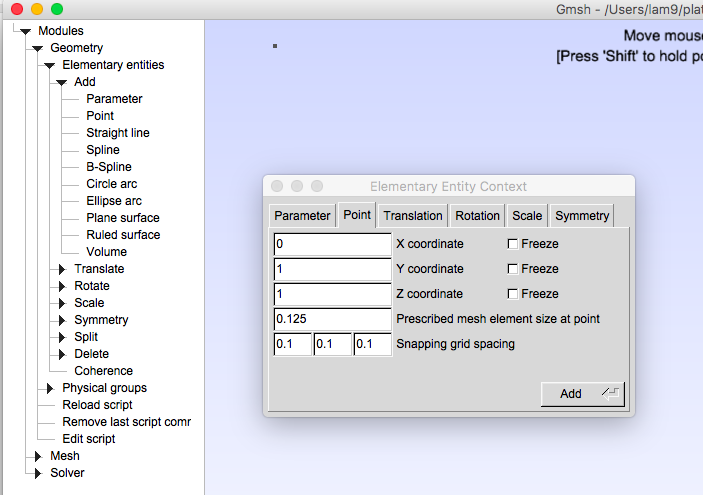
\includegraphics[width=0.95\textwidth]{ch22-gmsh-point.png}\\
The point dialog of the 2020 deck. Its ``Prescribed mesh element size'' reads $0.125$ in the screenshot while the text says $0.0625$; \code{plate2.msh} has elements about $0.07$ across, the text's value.
\end{columns}
\sourcecredit{Screenshot from the 2020 deck (Laura Miller, gmsh on macOS).}
\end{frame}

% 8
\begin{frame}{Making the plate in gmsh (2): extrude, volume, physical group}
\label{fr:gmsh2}
\footnotesize
\begin{columns}[T]
\column{0.5\textwidth}
\begin{enumerate}
  \setcounter{enumi}{3}
  \item \textbf{Elementary entities $\to$ Translate $\to$ Extrude surface}: $0.125$ in $x$; click the surface (it turns red), press \textbf{e}. ``This will make plate 2 elements thick.'' (The 2020 deck wrote \textbf{Add $\to$ Translate}; Extrude lives under Translate, not Add.)
  \item \textbf{Add $\to$ Volume}: click the dashed boundary of the slab, press \textbf{e}. (The extrusion already makes the volume; this step is harmless and redundant.)
  \item \textbf{Physical groups $\to$ Add $\to$ Volume}: click the yellow dot in the slab, press \textbf{e}; name it \code{plate2}. The name becomes the subdomain's name in libMesh (chapter 18).
\end{enumerate}
\column{0.48\textwidth}
\centering
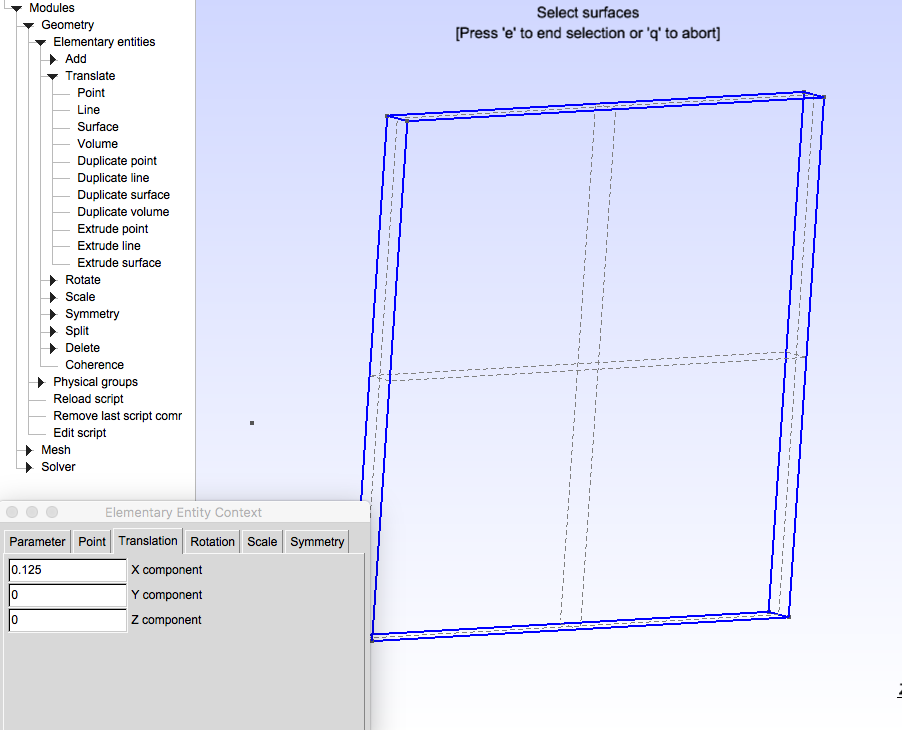
\includegraphics[width=0.49\textwidth]{ch22-gmsh-extrude.png}\hfill
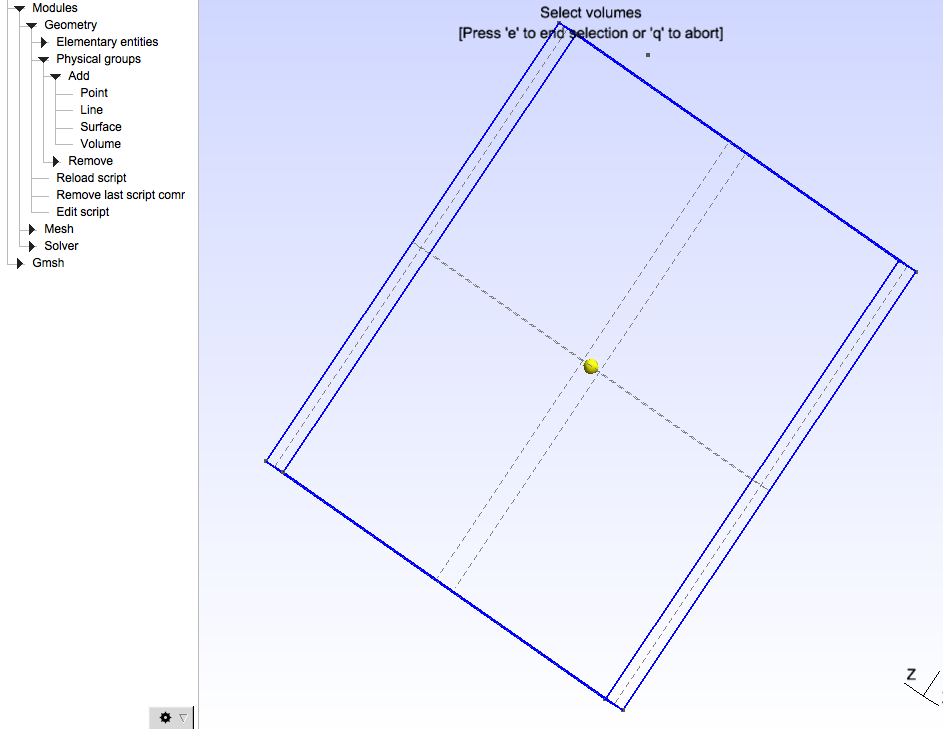
\includegraphics[width=0.49\textwidth]{ch22-gmsh-physical.png}\\
\scriptsize The extrude dialog ($0.125$ along $x$); the physical-volume pick (the yellow dot).
\end{columns}
\sourcecredit{Screenshots from the 2020 deck.}
\end{frame}

% 8b
\begin{frame}{Making the plate in gmsh (3): mesh and save}
\label{fr:gmsh3}
\scriptsize
\begin{columns}[T]
\column{0.55\textwidth}
\begin{enumerate}
  \setcounter{enumi}{6}
  \item \textbf{Mesh $\to$ 3D}, then \textbf{File $\to$ Save mesh}. ``This leaves only the 3D mesh and no 1D or 2D meshes that libmesh will reject'': with physical groups defined, gmsh saves only the elements that belong to one, so the lines and the surfaces stay out of the file.
\end{enumerate}
\begin{itemize}
  \item The deck's ``saves the mesh of the physical group as group\_name.msh'' is not right: the file takes the \emph{project's} name; you choose it in \textbf{File $\to$ Save as}. The physical group's name goes inside the file, as the subdomain's name.
  \item gmsh 4 saves MSH 4.1 by default; libMesh 1.7 reads MSH 2.2 and 4 as text, not binary. In \textbf{Save as} choose ``Version 2 ASCII'', or set \code{Mesh.MshFileVersion = 2.2} in a \code{.geo} file (chapter 18).
  \item The same seven steps as a script: a \code{.geo} with four \code{Point}s, four \code{Line}s, a \code{Line Loop}, a \code{Plane Surface}, \code{Extrude \{0.125, 0, 0\} \{ Surface\{1\}; \}} and \code{Physical Volume("plate2")}, then \code{gmsh -3 -format msh22 plate.geo}: chapter 18's route, which can be repeated and versioned.
\end{itemize}
\column{0.43\textwidth}
\centering
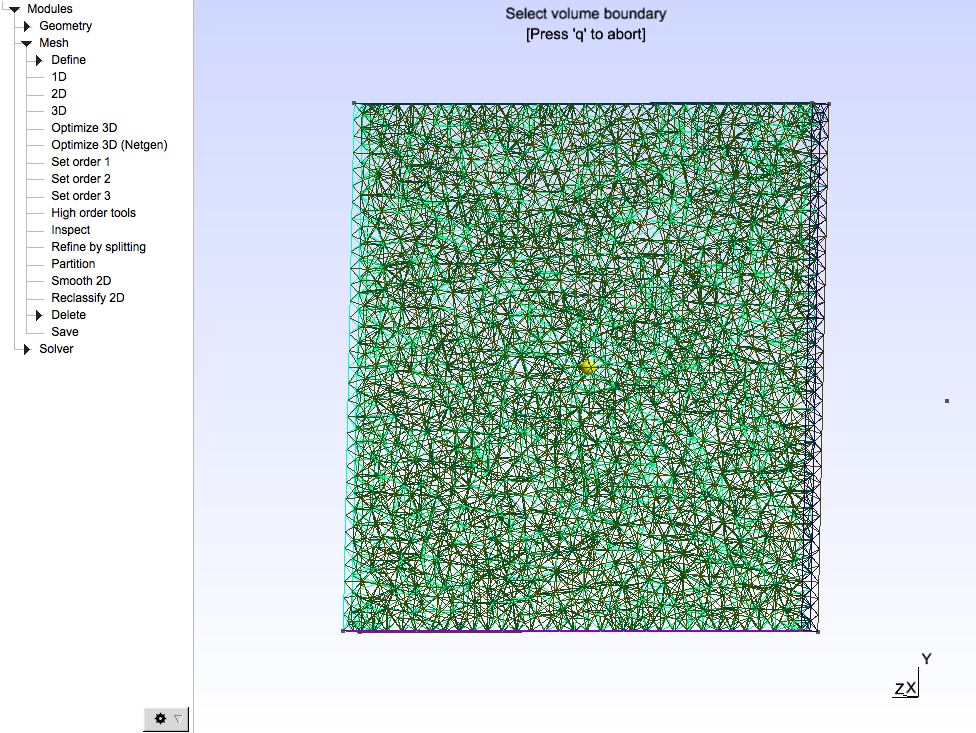
\includegraphics[width=0.85\textwidth]{ch22-gmsh-mesh.png}\\
\scriptsize The 3D mesh in gmsh (2020 deck): tetrahedra on the slab.
\end{columns}
\end{frame}

% 9
\begin{frame}{The mesh as libMesh reads it}
\label{fr:mesh}
\footnotesize
\begin{itemize}
  \item \code{plate2.msh}: MSH 2.2 text, $3386$ nodes, $11481$ elements of gmsh type $4$ (four-node tetrahedra, \code{TET4}), one physical volume \code{plate2}. Volume $0.5$: a tetrahedron of edge $h$ has volume $h^3/(6\sqrt2)$, so the mean edge is about $0.07$, the grid spacing, and there are two elements through the $0.125$ thickness.
  \item \code{MFAC} in the input (``ratio of Lagrangian mesh width to Cartesian mesh width'') does nothing here: it sizes meshes built in the program (IBAMR's \code{ex2}); a mesh read from a file is as fine as gmsh made it (chapter 18).
  \item Reading it: \code{mesh.read("plate2.msh")}, \code{mesh.prepare\_for\_use()}; the name comes from \code{MESH\_FILENAME} in the input. The 2017 deck noted ``the mesh name also appears in the main.C file, but I think those lines are obsolete''; the 2020 deck says it is ``given in both'': it is the input key's default value.
  \item With \code{IB\_point\_density = 1} and \code{QGRID}, each tetrahedron gets interaction points about $\mathrm{DX}$ apart (slide \ref{fr:input2}): about one per element here, which is what a body resolved by the grid needs; a body finer than the grid needs no more (chapter 17).
\end{itemize}
\end{frame}

% 9b
\begin{frame}{The mesh (2): the flat elements}
\label{fr:slivers}
\footnotesize
\begin{columns}[T]
\column{0.55\textwidth}
\begin{itemize}
  \item $80$ of the $11481$ tetrahedra have a shape quality below $0.05$ (a regular tetrahedron is $1$) and $4$ are below $0.01$: slivers that the extrusion's two layers of tetrahedra produce near the plate's faces.
  \item They are where $J = \det\mathbb{F}$ strays from $1$ in the run ($0.21$ to $2.1$ at $t = 0.5$ while the rest of the plate stays near $1$), and where a few nodes move $0.05$ when the plate's edge moves $0.01$ (slide \ref{fr:flaps}). A flat element has almost no volume, so a small displacement of one node changes its $J$ a lot; the stress there is large but acts on almost nothing, and the run survives. With a larger time step or a stiffer material, $J$ in a sliver goes negative first, $\ln J$ is undefined, and the run ends.
  \item \textbf{Mesh $\to$ Optimize 3D} in gmsh improves them; three layers instead of two avoid them; \code{Mesh.OptimizeNetgen = 1} in a \code{.geo} does it in a script. Chapter 16's checks (a short run, the range of $J$) catch them before a long run.
\end{itemize}
\column{0.43\textwidth}
\centering
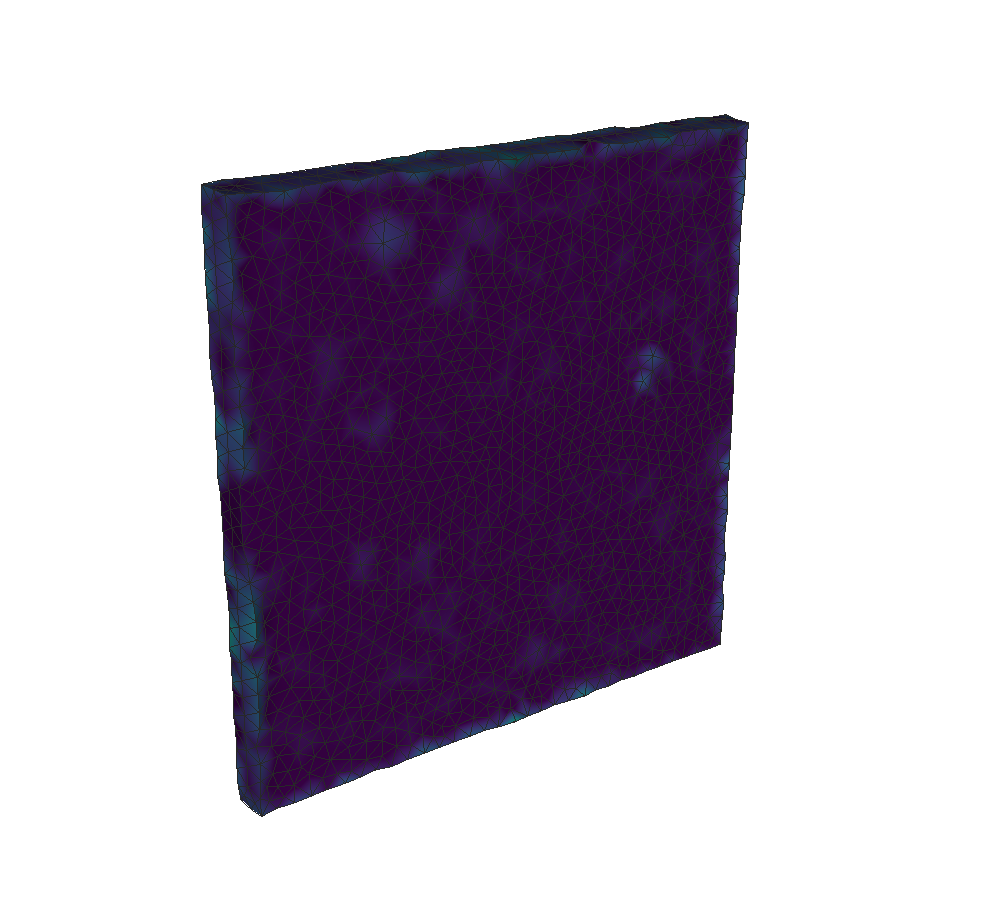
\includegraphics[width=0.9\textwidth]{ch22-plate-dx-outliers-t05.png}\\
\scriptsize The plate at $t = 0.5$ coloured by its downstream displacement on a scale to $0.05$: almost everything is dark (below $0.012$); the brighter spots are the sliver tetrahedra's nodes.
\end{columns}
\end{frame}

% 10
\begin{frame}[fragile]{The code (1): the tether band and the stress functions}
\label{fr:code1}
\begin{lstlisting}[style=cpptiny]
static double kappa_s = 1.0e5;  static double tether_half_width = 0.1;  static double translate_x = 0.0;   // from input3d
// Target ("tether") force on the plate, per unit reference volume. s is the reference position of a point of the
// plate (its position in the mesh file); X is where that point is now. Only the band |s(2)| < tether_half_width is tethered.
void target_force_function(VectorValue<double>& F, const TensorValue<double>& /*FF*/, const libMesh::Point& X,
                           const libMesh::Point& s, Elem* const /*elem*/, const std::vector<const std::vector<double>*>& /*var_data*/,
                           const std::vector<const std::vector<VectorValue<double> >*>& /*grad_var_data*/, double /*time*/, void* /*ctx*/)
{
    double kappa = 0.0;                                       // no tether force outside the band
    if (std::abs(s(2)) < tether_half_width) kappa = kappa_s;
    libMesh::Point s_target = s;                              // the tether location...
    s_target(0) += translate_x;                               // ...after the translation (none by default)
    F = kappa * (s_target - X);
}
void PK1_dev_stress_function(TensorValue<double>& PP, const TensorValue<double>& FF, ..., const libMesh::Point& s, ...)
{
    const bool leaf = two_materials && std::abs(s(2)) >= stem_half_width;
    const double mu = leaf ? mu_leaf : mu_stem;
    PP = mu * FF;
}
void PK1_dil_stress_function(TensorValue<double>& PP, const TensorValue<double>& FF, ..., const libMesh::Point& s, ...)
{
    const bool leaf = two_materials && std::abs(s(2)) >= stem_half_width;
    const double mu = leaf ? mu_leaf : mu_stem;  const double beta = leaf ? beta_leaf : beta_stem;
    const double J = FF.det();  J_minimum = std::min(J_minimum, J);  J_maximum = std::max(J_maximum, J);   // for output_data
    PP = (-1.0 * mu + beta * std::log(J)) * tensor_inverse_transpose(FF, NDIM);
}
\end{lstlisting}
\end{frame}

% 10b
\begin{frame}[fragile]{The code (1b): the tether in its three versions}
\label{fr:code1b}
\scriptsize
\begin{columns}[T]
\column{0.5\textwidth}
2017 (``main.C -- Target forces''; the old \code{system\_data} signature):
\begin{lstlisting}[style=cpptiny]
libMesh::Point s_dump;
double kappa;
s_dump = s; // this is the tether location before translation
s_dump(0) = s(0) - 7; // now the desired location is translated.
// apply tether force only if z-coordinate of original position is within 0.1 of center.
if (abs(s(2)) < .1) { kappa = kappa_s; }
else { // no tether force, set tether stiffness to zero.
       kappa = 0; }
F = kappa * (s_dump - X); // Note x is actual position, s_dump is desired position
\end{lstlisting}
2020 (slide 14; the translation gone, \code{s\_dump} left behind):
\begin{lstlisting}[style=cpptiny]
libMesh::Point s_dump;
double kappa;
s_dump = s;
if (abs(s(2)) < .1) { kappa = kappa_s; }
else { kappa = 0; }
F = kappa * (s - X); // Note x is actual position, s is desired position
\end{lstlisting}
\column{0.48\textwidth}
\begin{itemize}
  \item The stress functions are chapter 19's compressible neo-Hookean pair, with the material chosen by where the point is; the tether is chapter 19's body force restricted to a band of the reference configuration.
  \item ``Apply target force at the midline of plate using target\_force\_function. Applied in band running from $-.1$ to $.1$ in z-direction'' (2020, slide 13).
  \item The 2017 version is the right one when the plate is moved: the target is \code{s} \emph{shifted}, as the mapping shifted the mesh (slide \ref{fr:mapping2}). The 2020 version is right only because the mapping was removed with it.
  \item IBFE/10 keeps one function for both cases: \code{s\_target(0) += translate\_x}, with \code{translate\_x = 0} by default; the band width is an input key; \code{std::abs} replaces \code{abs}, which on some compilers truncates a double to an integer and makes every point ``inside''.
  \item The comment ``Note x is actual position'' names the variable \code{X}; the lower-case \code{x} in the 2017 and 2020 slides is a slip that survived three years.
\end{itemize}
\end{columns}
\end{frame}

% 11
\begin{frame}[fragile]{The code (2): the initial coordinate mapping}
\label{fr:mapping}
\footnotesize
\begin{columns}[T]
\column{0.5\textwidth}
IBFE/10:
\begin{lstlisting}[style=cpptiny]
// Initial coordinate mapping: where each point of the mesh starts.
// s is the position in the mesh file and X is the starting position in the fluid.
void coordinate_mapping_function(libMesh::Point& X, const libMesh::Point& s, void* /*ctx*/)
{
    X(0) = s(0) + translate_x;
    X(1) = s(1);
    X(2) = s(2);
}
...
if (ModelData::translate_x != 0.0)
{
    ib_method_ops->registerInitialCoordinateMappingFunction(coordinate_mapping_function);
}
ib_method_ops->initializeFEEquationSystems();
\end{lstlisting}
\column{0.48\textwidth}
The 2017 deck (slide 13, ``main.C -- Translate FE boundary''): ``We made our FE mesh at the origin. We want to shove the plate left so it's at the beginning of the flow tank. The coordinate\_mapping\_function does this'':
\begin{lstlisting}[style=cpptiny]
void coordinate_mapping_function(libMesh::Point& X, const libMesh::Point& s, void* /*ctx*/)
{
    X(0) = s(0) - 7; // translated 7 units left along x-axis
    return;
}
...
ib_method_ops->registerInitialCoordinateMappingFunction(coordinate_mapping_function);
\end{lstlisting}
\begin{itemize}
  \item The signature: the starting position \code{X} to fill, the file's \code{s}, and \code{ctx}. Chapter 21's two-plate example used it to turn a plate upright and place two copies; chapter 17 introduced it with the rotated plate.
\end{itemize}
\end{columns}
\end{frame}

% 11b
\begin{frame}{The coordinate mapping (2): what it does, and what must follow it}
\label{fr:mapping2}
\footnotesize
\begin{itemize}
  \item \al{What it does.} Before the first step, IBFE sets every node's position $\mathbf{X}$ from its file coordinates $\mathbf{s}$ through this function (the default is $\mathbf{X} = \mathbf{s}$). Only $\mathbf{X}$ moves afterwards; $\mathbf{s}$ stays the file's coordinates for the whole run and in every callback: the stress functions, the forces, the post-processing.
  \item \al{So the tether must be mapped too.} A target of \code{s} pulls the plate back to the file's position. The 2017 code wrote \code{s\_dump(0) = s(0) - 7} in the tether; IBFE/10 adds \code{translate\_x} to \code{s\_target}. Any function that compares $\mathbf{X}$ to $\mathbf{s}$ (a tether, a prescribed motion, chapter 21's two copies) needs the same mapping; a material chosen by $\mathbf{s}$ does not, because the file's coordinates still say where in the body a point is.
  \item \al{Set every component.} The 2017 function set \code{X(0)} only; \code{X} arrives holding $\mathbf{s}$, so that works, but write all three (IBFE/10) and nobody has to know.
  \item \al{\code{dX} in the output} is $\mathbf{X} - \mathbf{s}$: it includes the shift. In VisIt the displaced mesh is in the right place; a plot of \code{dX\_0} on a plate moved by $4$ reads about $4$ everywhere, and the bend is the small variation on top.
  \item \al{Register before} \code{initializeFEEquationSystems()}, once per part (\code{..., part)} for several); a mapping registered later is ignored.
  \item \al{A rotation} is the same mechanism: $\mathbf{X} = R\,\mathbf{s}$ with a rotation matrix $R$, and the tether target $R\,\mathbf{s}$. The horseshoe crab's ``$0$ degrees'' (slide \ref{fr:crab}) is where that goes.
\end{itemize}
\end{frame}

% 12
\begin{frame}{The coordinate mapping (3): ``not working as it used to'', re-tested}
\label{fr:mapping3}
\scriptsize
\begin{itemize}
  \item The 2020 deck dropped the translation: ``Previously, we translated the plate to the left. That feature is not working as it used to in newer versions of IBAMR'' (slide 3), moved the tank from $-16 < x < 16$ to $-8 < x < 24$ instead, and commented the registration out (\code{//ib\_method\_ops->registerInitialCoordinateMappingFunction(...)} in the course's \code{main.C}).
  \item \al{What the 2017 input actually said.} Its slide 3 reads ``The domain goes from $-16 < x < 16$ \ldots translate 7 units in the negative x-direction''. But the \code{input3d} in the 2017 zip already has \code{x\_lo = -0.5*L}, \code{x\_up = 1.5*L}: the tank was $-8 < x < 24$ then too, and the plate shifted by $-7$ stood \emph{one unit} from the inflow face, inside the kernel's reach of the boundary where the velocity is prescribed. A plate that cannot move its fluid is a plausible ``not working''.
  \item \al{Re-tested with IBAMR 0.19.0.} \code{TRANSLATE\_X = 4.0} (the plate $12$ units from the inflow face), run to $t = 0.1$: the plate sits at $x = 4$ (its mean $x$ in \code{output.ex2} is $4.06$), and the tether force at $t = 0.1$ is the same as in the default run to four digits ($-0.1064$ against $-0.1064$). The mapping works; in a tank this large the plate's position hardly matters.
  \item \al{When to use it.} One mesh file, many placements: an angle of attack, a position in the tank, chapter 21's second copy. The alternative, editing the mesh in gmsh, changes a file that others share.
\end{itemize}
\begin{punchbox}
\scriptsize Rule: map \code{s} wherever the code compares positions, and keep the body away from a face where the velocity is prescribed: at least a few kernel widths, and much more if its wake must leave through the outflow.
\end{punchbox}
\end{frame}

% 13
\begin{frame}[fragile]{The 2017 two-material plate}
\label{fr:twomat}
\scriptsize
\begin{columns}[T]
\column{0.5\textwidth}
``Let the plate have 2 stiffnesses (middle half is different than ends)'' (2017, slide 2); in the code the band is $|s_2| < 0.25$, the middle \emph{quarter}:
\begin{lstlisting}[style=cpptiny]
// 2017 main.C
if (abs(s(2)) < .25) { mu = mu_stem; beta = beta_stem; }
else                 { mu = mu_leaf; beta = beta_leaf; }
// 2017 input3d
NU=0.3
E_STEM=7000
E_LEAF=140000
MU_LEAF = E_STEM/(2.0*(1.0+NU))     // 1e2
MU_STEM = E_LEAF/(2.0*(1.0+NU))     // 1e5
BETA_STEM = (E_STEM*NU) / ((1.0 + NU)*(1.0 - 2.0*NU))
BETA_LEAF = E_LEAF*NU/((1.0 + NU)*(1.0 - 2.0*NU))
KAPPA_S = 1e6
\end{lstlisting}
\begin{itemize}
  \item $\mu = E/(2(1+\nu))$ and $\beta = E\nu/((1+\nu)(1-2\nu))$ are the shear modulus and the first Lam\'e parameter of a linear solid with Young's modulus $E$ and Poisson's ratio $\nu$: the way to choose a neo-Hookean material's two constants from numbers you can look up.
\end{itemize}
\column{0.48\textwidth}
\begin{itemize}
  \item \al{The swap.} Since 2017 the two \code{MU} lines use each other's $E$ (\code{MU\_STEM} from \code{E\_LEAF}) while the \code{BETA} lines use their own, and the comments ($10^2$, $10^5$) match neither. IBFE/10 keeps the swap so its runs match the course's: the plate has $\mu_s = 0.538$ ($E = 1.4$) and $\beta = 0.404$ ($E = 0.7$), which together correspond to $E \approx 1.31$, $\nu \approx 0.21$. Fix it for your own runs.
  \item \al{Restored as an input option.} \code{TWO\_MATERIALS = TRUE} with \code{STEM\_HALF\_WIDTH = 0.25}: stem $\mu = 0.538$, $\beta = 0.404$; leaf $\mu = 0.269$, $\beta = 0.808$ (the softer flaps). Run to $t = 0.1$ with 0.19.0: the force on the plate is $9\%$ smaller ($-0.097$ against $-0.106$), the flap edges have moved the same $0.001$, and $J$ ranges further ($0.64$ to $2.96$).
  \item Choosing the material by \code{s} is chapter 19's ``a stress that depends on where you are''; a subdomain id from gmsh's physical groups (chapter 18) does the same without a coordinate test.
\end{itemize}
\end{columns}
\end{frame}

% 14
\begin{frame}[fragile]{The input file (1): grid, time and output}
\label{fr:input}
\footnotesize
\begin{columns}[T]
\column{0.5\textwidth}
\begin{lstlisting}[style=inputtiny]
L = 16.0                 // width of the domain
MAX_LEVELS = 3
REF_RATIO  = 4
N = 16                   // cells across the width on level 0
NFINEST = (REF_RATIO^(MAX_LEVELS - 1))*N    // 256
DX  = L/NFINEST          // 0.0625
MFAC = 3.0               // no effect: the mesh is a file
PK1_DEV_QUAD_ORDER = "SEVENTH"
PK1_DIL_QUAD_ORDER = "FIFTH"
KAPPA_S = 1e5
TETHER_HALF_WIDTH = 0.1
TRANSLATE_X = 0.0
TWO_MATERIALS = FALSE
STEM_HALF_WIDTH = 0.25
...
DT                         = 1e-4
CFL_MAX                    = 0.2
END_TIME                   = 0.5    // the course: 2.0
VIZ_INTERVAL     = int(END_TIME/(20*DT))   // 21 frames
DATA_INTERVAL    = int(END_TIME/(100*DT))  // 100 lines
RESTART_INTERVAL = int(0.5/DT + 0.5)
GriddingAlgorithm {
   ratio_to_coarser {
      level_1 = REF_RATIO,REF_RATIO,REF_RATIO ... }
   largest_patch_size { level_0 = 256,256,256 }
   smallest_patch_size { level_0 = 8,8,8 } ... }
\end{lstlisting}
\column{0.48\textwidth}
\scriptsize
\begin{itemize}
  \item Three refinement ratios per level, three sizes per patch; \code{largest\_patch\_size} $256^3$ lets one patch hold a whole level.
  \item \code{vorticity\_abs\_thresh = 0.125,0.25,.5,1,2} tags cells for refinement where $|\boldsymbol\omega|$ exceeds the level's threshold; with $\mathrm{Re} = 20$ the vorticity is weak and the plate's own cells (tagged because they hold Lagrangian points) decide most of the fine level (slide \ref{fr:levels}).
  \item \code{PK1\_*\_QUAD\_ORDER} are the stress quadrature orders of chapter 19 (\code{SEVENTH} and \code{FIFTH} here, \code{THIRD} by default); for linear tetrahedra and a smooth stress they are generous.
  \item $\mathrm{DT} = 10^{-4}$ with $\mathrm{DX} = 1/16$ and $U = 0.1$ is a CFL of $0.00016$: the limit is the tether, $\kappa_s = 10^5$, not the flow (chapter 19, slide 26).
  \item The intervals are written in terms of \code{END\_TIME} and \code{DT}, so a longer run keeps $20$ frames and $100$ force lines; the course's \code{int(0.1/DT)} gave $20$ frames for its $2$ time units.
\end{itemize}
\end{columns}
\end{frame}

% 14b
\begin{frame}[fragile]{The input file (2): the IBFE interaction keys}
\label{fr:input2}
\footnotesize
\begin{columns}[T]
\column{0.42\textwidth}
\begin{lstlisting}[style=inputtiny]
IB_DELTA_FUNCTION          = "IB_4"
SPLIT_FORCES               = FALSE
USE_JUMP_CONDITIONS        = FALSE
USE_CONSISTENT_MASS_MATRIX = TRUE
IB_POINT_DENSITY           = 1.0
...
IBFEMethod {
   IB_delta_fcn               = IB_DELTA_FUNCTION
   split_forces               = SPLIT_FORCES
   use_jump_conditions        = USE_JUMP_CONDITIONS
   use_consistent_mass_matrix = USE_CONSISTENT_MASS_MATRIX
   IB_point_density           = IB_POINT_DENSITY
   IB_quad_type               = "QGRID"   // or "QGAUSS"
}
\end{lstlisting}
\column{0.56\textwidth}
\scriptsize
\setlength{\tabcolsep}{3pt}
\begin{tabular}{@{}L{0.36\textwidth}L{0.6\textwidth}@{}}
\toprule
key (read by \code{getFromInput}) & what it sets \\
\midrule
\code{IB\_delta\_fcn} & the kernel for interpolation and spreading (\code{IB\_4} here; chapter 17) \\
\code{IB\_point\_density} & interaction points per $\mathrm{DX}$ along each direction of an element: $1$ gives about one point per $\mathrm{DX}$, $2$ twice as many \\
\code{IB\_quad\_type}, \code{IB\_quad\_order} & the rule that places them: \code{QGRID} on a grid inside the element (adaptive to the density), \code{QGAUSS} at Gauss points of the given order \\
\code{IB\_use\_nodal\_}\newline\code{quadrature} & the nodes themselves as interaction points, with a lumped mass matrix (\code{QTRAP}, first order) \\
\code{interp\_*}, \code{spread\_*} & the same keys for interpolation and spreading separately; \code{IB\_*} sets both \\
\code{split\_forces},\newline\code{use\_jump\_conditions} & the boundary-term treatment of chapter 19, slide 7 \\
\code{use\_consistent\_}\newline\code{mass\_matrix} & the $L^2$ projection of the velocity onto the mesh: consistent (a solve) or lumped \\
\bottomrule
\end{tabular}
\end{columns}
\end{frame}

% 15
\begin{frame}[fragile]{Running it}
\label{fr:run}
\footnotesize
\begin{columns}[T]
\column{0.5\textwidth}
\begin{lstlisting}[style=shell]
# laptop (autoibamr); on Puma add: module load gnu13 openmpi5
source ~/autoibamr/configuration/enable.sh
cmake -S . -B build -DCMAKE_BUILD_TYPE=Release
cmake --build build -j 4
mpirun -np 4 ./build/main3d input3d
# continue a finished run from its restart files:
mpirun -np 4 ./build/main3d input3d restart_IB3d 5000
\end{lstlisting}
\begin{itemize}
  \item On Puma the modules load only on compute nodes: build and run inside an interactive session or the batch job (\code{job.slurm}: 4 cores, the \code{standard} partition); chapter 31.
  \item The restart line continues from step $5000$ with the finite element data of the plate reloaded and \code{output.ex2} appended (chapter 21's rule).
\end{itemize}
\column{0.48\textwidth}
\begin{tabular}{@{}L{0.5\textwidth}L{0.44\textwidth}@{}}
\toprule
$5000$ steps, 4 cores (laptop, WSL) & $3096$ s: $0.62$ s per step \\
the course's $2$ time units & $20000$ steps: about $3.5$ hours \\
\code{viz\_IB3d/} ($21$ frames of $4.4$ MB, plus \code{output.ex2}, $7.2$ MB) & about $100$ MB \\
restart files at the end & $10$ MB; the folder $115$ MB \\
0.16.0 and 0.19.0 & the same tether force to all six digits at $t = 0.5$ \\
\bottomrule
\end{tabular}
\end{columns}
\end{frame}

% 15b
\begin{frame}{What a 3D run costs}
\label{fr:cost}
\footnotesize
\begin{itemize}
  \item Why $0.6$ s per step: three levels of a $32\times16\times16$ base, $11481$ elements with a point density of $1$, and a staggered-grid solve of the whole tank every step. IBFE/08's 2D plate took $15$ ms per step. The cell count grows as $\mathrm{DX}^{-3}$, and the work as $\mathrm{DX}^{-4}$ once the time step shrinks with the cells.
  \item Before a long run: a short one (\code{END\_TIME = 0.002}, $20$ steps, the ``smoke test'') to see that the files appear and the force line prints; then a run to $0.1$ to time it; then the real one, in a batch job, with restart files written on the way (\code{RESTART\_INTERVAL}).
  \item The course's \code{data\_dump\_interval = 1} called an empty \code{output\_data} every step and printed ``Max Jacobian 1'' that never changed; IBFE/10 computes the tether force $100$ times per run and prints the real range of $J$.
  \item Output per frame is the whole hierarchy: keep \code{VIZ\_INTERVAL} coarse and use restarts for the rest. Forty frames of this run are $180$ MB; the course's twenty frames of a tank at $\mathrm{DX} = 1/32$ would be eight times that.
  \item The horseshoe crab (slide \ref{fr:crab}) is the other end: $50000$ steps on $64$ cores for up to $72$ hours.
\end{itemize}
\end{frame}

% 16
\begin{frame}{What you should see (1): the tether force}
\label{fr:force}
\scriptsize
\begin{columns}[T]
\column{0.46\textwidth}
Every $50$ steps the screen shows
\begin{center}\tiny\code{tether force = -0.106699 0.00112701 0.00150725   J from 0.822529 to 1.72649}\end{center}
the total tether force on the plate and the range of $J$ since the last line; the force goes to \code{hier\_data\_IB3d/tether\_force.txt}.

\medskip
\begin{tabular}{@{}llll@{}}
\toprule
$t$ & $U(t)$ & $F_x$ & $J$ range \\
\midrule
$0.05$ & $0.010$ & $-0.107$ & $0.82$--$1.73$ \\
$0.10$ & $0.020$ & $-0.106$ & $0.66$--$2.51$ \\
$0.15$ & $0.029$ & $-0.150$ & \\
$0.20$ & $0.038$ & $-0.192$ & $0.35$--$2.72$ \\
$0.25$ & $0.046$ & $-0.194$ & \\
$0.30$ & $0.054$ & $-0.215$ & $0.52$--$2.14$ \\
$0.35$ & $0.060$ & $-0.221$ & \\
$0.40$ & $0.066$ & $-0.239$ & \\
$0.45$ & $0.072$ & $-0.263$ & \\
$0.50$ & $0.076$ & $-0.276$ & $0.21$--$2.10$ \\
\bottomrule
\end{tabular}
\column{0.52\textwidth}
\begin{itemize}
  \item The tether is what holds the plate against the stream, so minus the tether force is the force of the fluid on the plate: $F_x$ is minus the drag (once the flaps have stopped bending, on the whole plate; before that, on the band plus what the flaps hand to it).
  \item \al{An accelerating stream pushes before it flows.} At $t = 0.05$ the stream is at a tenth of its speed and the force is already $0.107$, $40\%$ of its value at $t = 0.5$: the fluid around the plate is accelerating ($\dot U = 2U\,\mathrm{sech}^2 2t$, $0.2$ at the start) and the plate must push it. That force falls as $\dot U$ falls (to $0.084$ at $t = 0.5$) while the steady drag rises with $U$; the sum is what the table shows. A run that starts the stream impulsively sees this force in one step, with the tether stiffness deciding how large.
  \item $F_y$ and $F_z$ are $0.036$ and $-0.015$ at $t = 0.5$: the plate is not quite symmetric (the mesh is not), and the top flap bends a little more than the bottom one.
  \item 0.16.0 and 0.19.0 give the same ten lines to four digits.
\end{itemize}
\end{columns}
\end{frame}

% 17
\begin{frame}{What you should see (2): the flaps}
\label{fr:flaps}
\scriptsize
\begin{columns}[T]
\column{0.5\textwidth}
From \code{output.ex2} (the free edges are the nodes at $z = \pm1$ in the mesh file):
\begin{tabular}{@{}llll@{}}
\toprule
$t$ & top edge $\Delta x$ & bottom edge $\Delta x$ & band \\
\midrule
$0.1$ & $0.0011$ & $0.0010$ & $< 3\times10^{-5}$ \\
$0.2$ & $0.0040$ & $0.0035$ & \\
$0.3$ & $0.0076$ & $0.0065$ & \\
$0.4$ & $0.0102$ & $0.0085$ & \\
$0.5$ & $0.0116$ & $0.0094$ & $< 3\times10^{-5}$ \\
\bottomrule
\end{tabular}
\begin{itemize}
  \item The flaps bend downstream slowly: $0.012$ at the edge of a flap $1$ long is a small bend, as $\mu_s = 0.54$ against a dynamic pressure of $\rho U^2/2 = 0.003$ predicts. The top flap bends a little more. The tethered band does not move.
  \item A few nodes move up to $0.05$: the sliver tetrahedra of slide \ref{fr:slivers}, which are also where $J$ strays. They are a mesh defect, not a flow feature.
  \item Softer flaps (\code{E\_STEM = 0.07}) or a faster stream bend more; the course's run to $t = 2$ reaches the steady stream and a steady bend.
\end{itemize}
\column{0.48\textwidth}
\centering
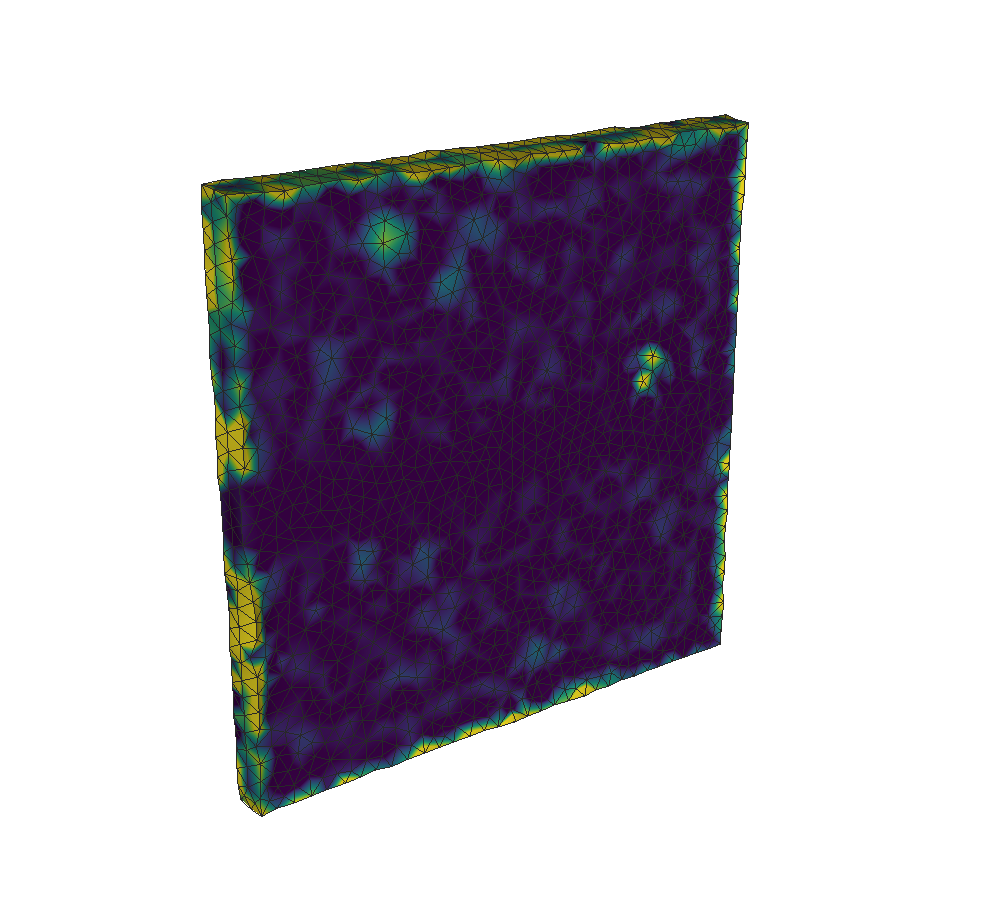
\includegraphics[width=0.78\textwidth]{ch22-plate-dx-t05.png}\\
The plate at $t = 0.5$, coloured by its downstream displacement \code{dX\_0} ($0$ to $0.012$), at true displacement, seen from downstream: the free edges have moved most.
\end{columns}
\end{frame}

% 18
\begin{frame}{What you should see (3): the flow}
\label{fr:flow}
\begin{columns}[T]
\column{0.5\textwidth}\centering
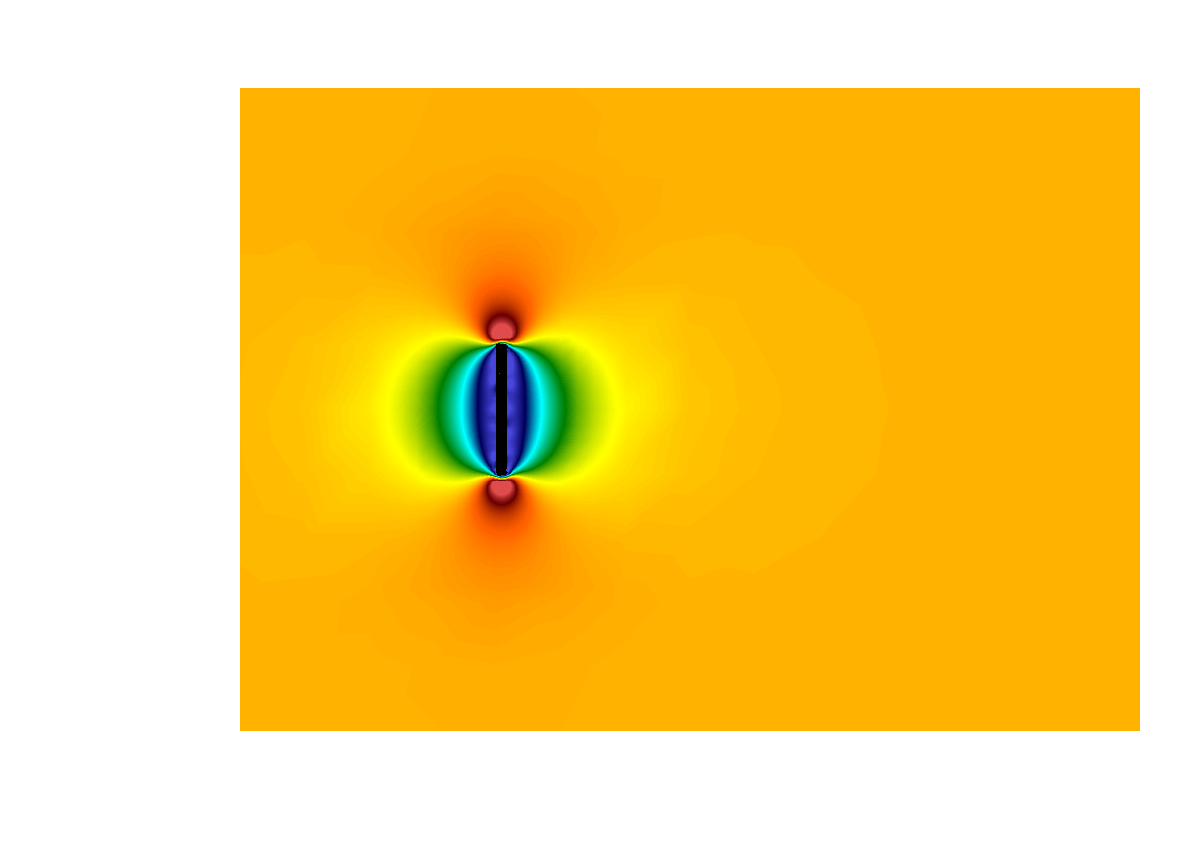
\includegraphics[width=0.86\textwidth]{ch22-ux-slice-t05.png}\\
\scriptsize $u_x$ ($0$ to $0.12$) on the slice $y = 0$ at $t = 0.5$; $-4 < x < 10$. The plate's cross-section in black.
\column{0.5\textwidth}\centering
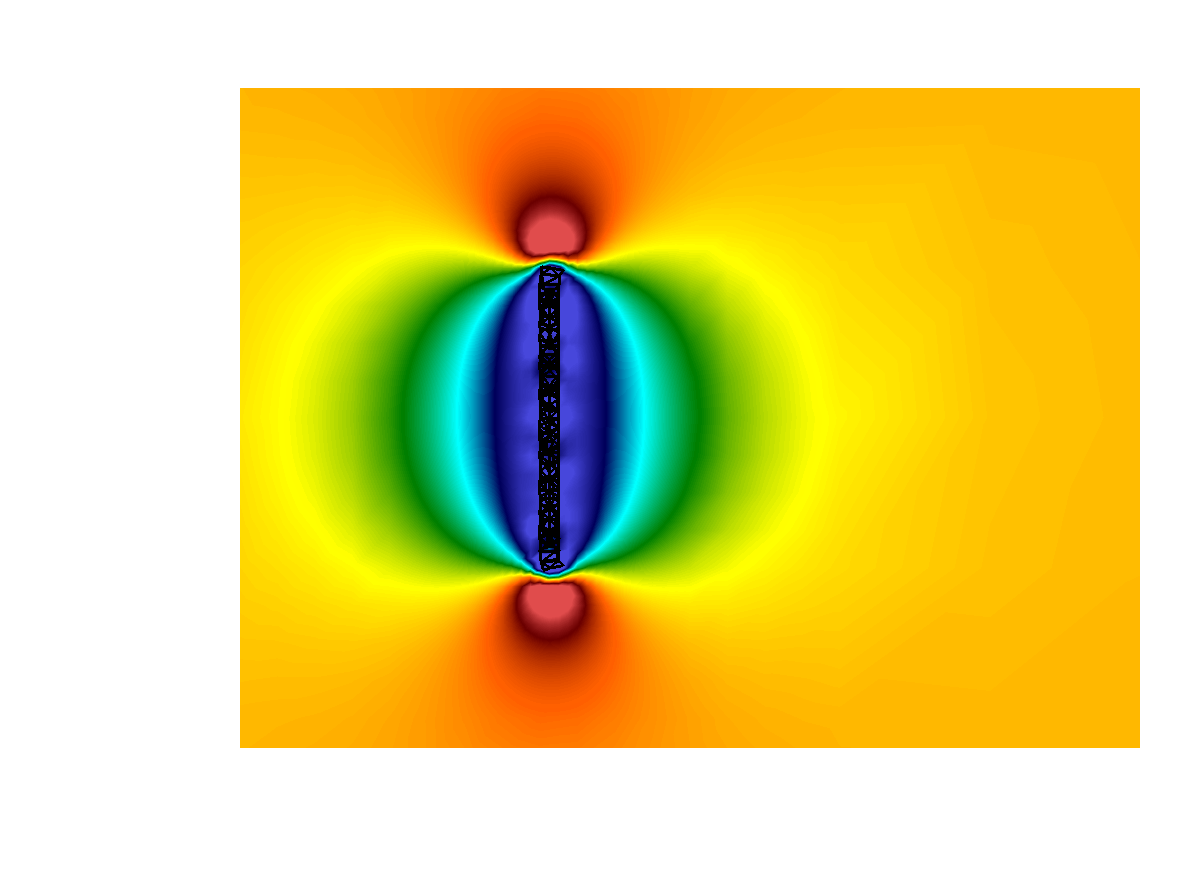
\includegraphics[width=0.86\textwidth]{ch22-ux-slice-zoom-t05.png}\\
\scriptsize The same, $-2 < x < 4$: the stream goes round the plate's edges, a slow wake behind it.
\end{columns}
\scriptsize
\begin{itemize}
  \item At $\mathrm{Re} = 20$ there is no shedding: a steady recirculation forms behind the plate and the wake recovers within a few plate widths. The slice is the $x$--$z$ plane through the tethered band's middle, so it cuts the band and both flaps.
  \item Ahead of the plate the fluid slows (stagnation); above and below its edges it speeds up to $0.12$, above the stream's $0.076$.
\end{itemize}
\sourcecredit{IBFE/10, IBAMR 0.19.0 (\code{/root/work/0.19.0/runs/ft\_default}); \code{wsl/final/visit\_ch22.sh}.}
\end{frame}

% 19
\begin{frame}{What you should see (4): vorticity, the 3D view, and the course's own picture}
\label{fr:flow2}
\begin{columns}[T]
\column{0.33\textwidth}\centering
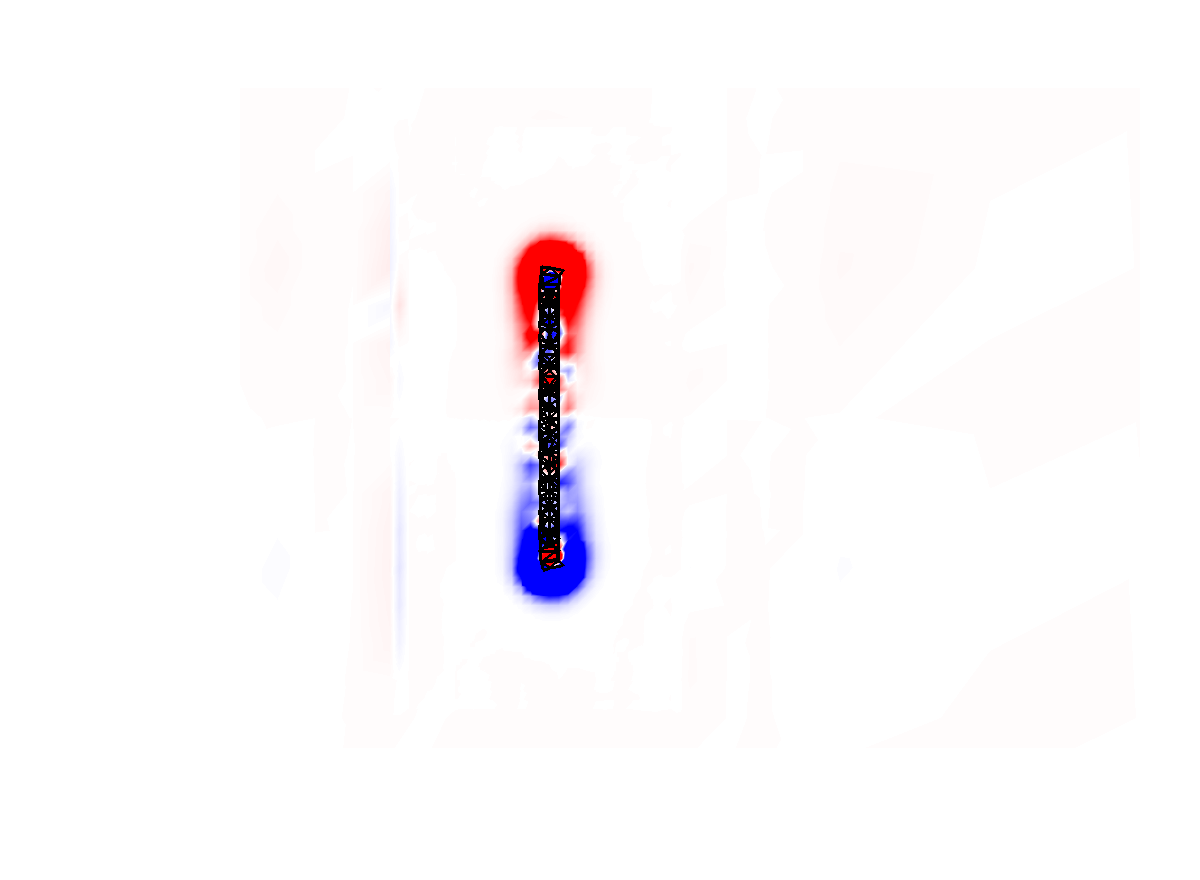
\includegraphics[width=\textwidth]{ch22-vort-slice-zoom-t05.png}\\
\scriptsize $\omega_y$ ($\pm0.3$) on the slice $y = 0$: vorticity of opposite sign shed from the plate's two edges.
\column{0.33\textwidth}\centering
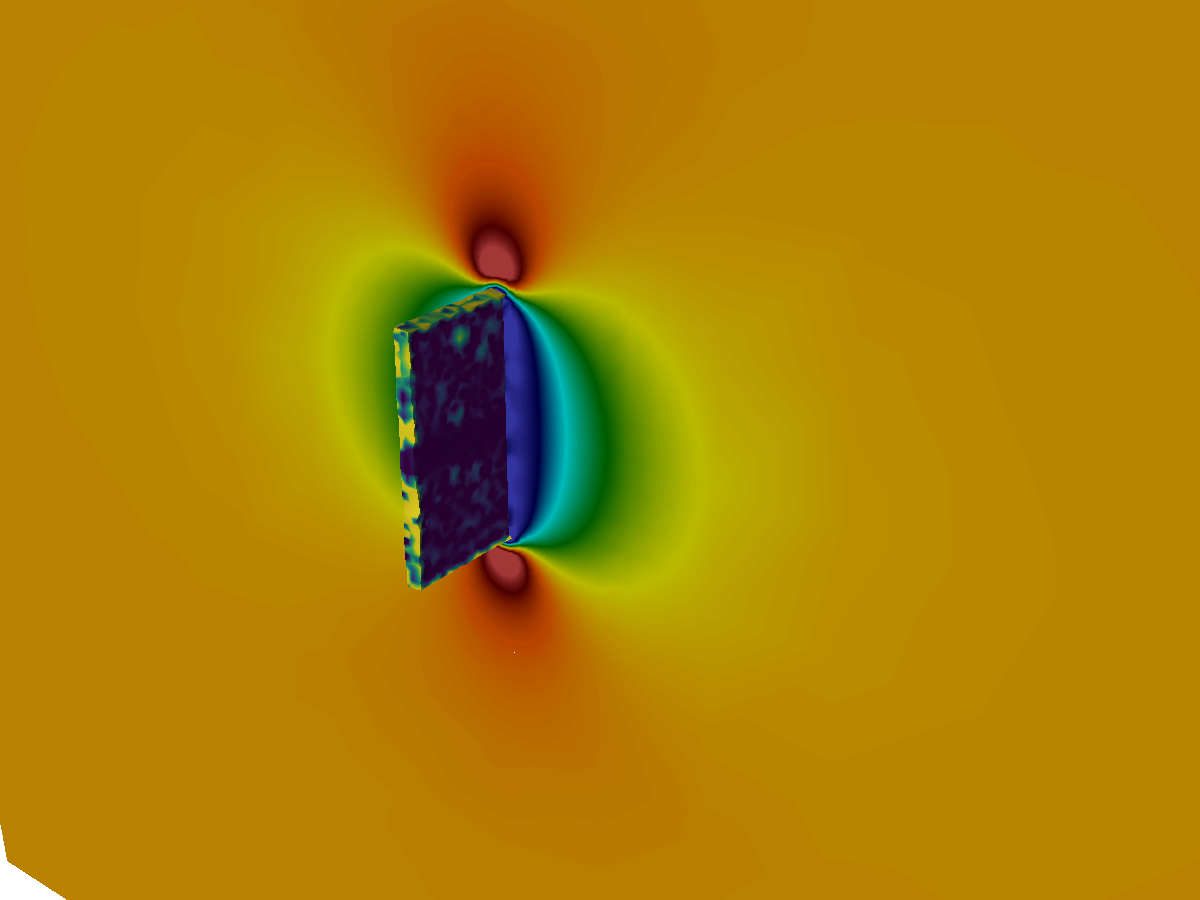
\includegraphics[width=\textwidth]{ch22-3d-t05.png}\\
\scriptsize The slice in 3D with the displaced plate coloured by \code{dX\_0}.
\column{0.33\textwidth}\centering
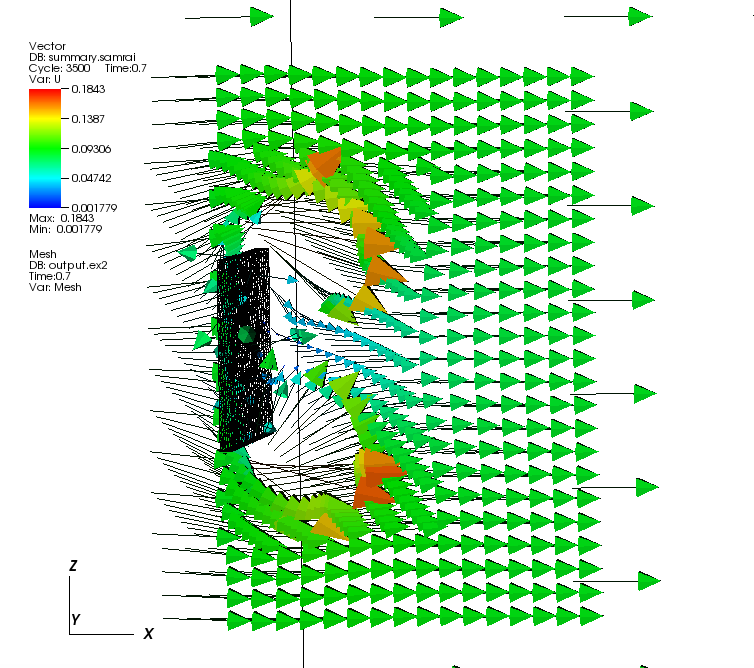
\includegraphics[width=0.85\textwidth]{ch22-2020-render.png}\\
\scriptsize The 2020 deck's render (slide 2): velocity vectors on a slice at $t = 0.7$ of the course's run, the plate's mesh in black.
\end{columns}
\scriptsize
\begin{itemize}
  \item In 3D the vorticity is a vector; the 2D decks' \code{Omega} is its component normal to the plane you look at, \code{Omega[1]} on this slice, and \code{magnitude(Omega)} is the scalar for a 3D view.
  \item The course's picture shows the same flow $0.2$ later: the vectors bend round the plate and the recirculation behind it shows in the vectors that point upstream.
\end{itemize}
\end{frame}

% 20
\begin{frame}{The grid: three levels}
\label{fr:levels}
\begin{columns}[T]
\column{0.55\textwidth}\centering

\includegraphics[width=\textwidth]{ch22-levels-slice-t05.png}\\
\scriptsize The tank on the slice $y = 0$ at $t = 0.5$: level 0 (red, $\mathrm{DX} = 1$), level 1 (green, $1/4$), level 2 (blue, $1/16$). The plate's section is the black line inside the blue box.
\column{0.43\textwidth}
\footnotesize
\begin{itemize}
  \item The finest level is a box round the plate and its near wake; the rest of the tank is $1$ and $1/4$ coarse. With $\mathrm{Re} = 20$ the vorticity thresholds tag little; the Lagrangian points tag the plate's cells, and \code{tag\_buffer = 1} pads them.
  \item If the whole tank were at $\mathrm{DX} = 1/16$ it would be $512\times256\times256 = 33$ million cells; the three levels keep it to a few hundred thousand.
\end{itemize}
\end{columns}
\end{frame}

% 20b
\begin{frame}{The grid (2): what to adjust}
\label{fr:levels2}
\footnotesize
\begin{itemize}
  \item A wake that leaves the blue box is computed on the coarser level, with the $1/4$ spacing: fine at this Reynolds number, not at a higher one. The thresholds (\code{vorticity\_abs\_thresh}, one per level) and so the box the fine level covers are what you adjust; chapter 16's convergence study says when it is enough.
  \item \code{regrid\_cfl\_interval = 0.5}: the hierarchy is rebuilt whenever a point could have moved half a cell; for a plate that barely moves that happens a few times per run (three regrids in this run's log). A body that swims regrids often, and each regrid costs a few steps' worth of time.
  \item \code{tag\_buffer = 1} pads every tagged region by one cell of the coarser level; a larger buffer keeps a moving body inside its fine box longer between regrids.
  \item The ratio $4$ between levels is IBAMR's usual choice: $16$ cells of the fine level for one coarse cell in 2D, $64$ in 3D. A ratio of $2$ with more levels refines more gradually at the price of more levels to manage.
  \item A finer base grid ($N = 32$) with the same three levels doubles the resolution everywhere and costs eight times the cells and sixteen times the work; a fourth level costs only where it is placed.
\end{itemize}
\end{frame}

% 21
\begin{frame}[fragile]{The post-processing (1): the tether force as an integral over the plate}
\label{fr:output}
\begin{lstlisting}[style=cpptiny,basicstyle=\ttfamily\fontsize{5.6}{6.6}\selectfont\color{BlackGray}]
void output_data(..., Mesh& mesh, EquationSystems* equation_systems, const std::string& coords_system_name,
                 const int iteration_num, const double loop_time, const string& data_dump_dirname)
{
    System& X_system = equation_systems->get_system(coords_system_name);          // the current positions X
    NumericVector<double>* X_ghost_vec = X_system.current_local_solution.get();  copy_and_synch(*X_system.solution, *X_ghost_vec);
    const DofMap& dof_map = X_system.get_dof_map();  std::vector<std::vector<unsigned int> > dof_indices(NDIM);
    std::unique_ptr<FEBase> fe(FEBase::build(dim, dof_map.variable_type(0)));
    std::unique_ptr<QBase> qrule = QBase::build(QGAUSS, dim, FIFTH);  fe->attach_quadrature_rule(qrule.get());
    const std::vector<double>& JxW = fe->get_JxW();  const std::vector<libMesh::Point>& q_point = fe->get_xyz();
    const std::vector<std::vector<double> >& phi = fe->get_phi();
    double F_integral[NDIM] = {0.0, 0.0, 0.0};  VectorValue<double> F;  libMesh::Point X;  boost::multi_array<double, 2> X_node;
    for (auto el_it = mesh.active_local_elements_begin(); el_it != mesh.active_local_elements_end(); ++el_it)
    {
        Elem* const elem = *el_it;  fe->reinit(elem);  for (unsigned int d = 0; d < NDIM; ++d) dof_map.dof_indices(elem, dof_indices[d], d);
        get_values_for_interpolation(X_node, *X_ghost_vec, dof_indices);
        for (unsigned int qp = 0; qp < qrule->n_points(); ++qp)
        {
            interpolate(X, qp, X_node, phi);                      // X at the quadrature point; q_point[qp] is s there
            target_force_function(F, FF_unused, X, q_point[qp], elem, var_data, grad_var_data, loop_time, nullptr);
            for (unsigned int d = 0; d < NDIM; ++d) F_integral[d] += F(d) * JxW[qp];
        }
    }
    IBTK_MPI::sumReduction(F_integral, NDIM);
    const double J_min = IBTK_MPI::minReduction(J_minimum);  const double J_max = IBTK_MPI::maxReduction(J_maximum);  // then reset
    pout << "tether force =";  for (unsigned int d = 0; d < NDIM; ++d) pout << " " << F_integral[d];  pout << "   J from " << J_min << " to " << J_max << "\n";
    if (IBTK_MPI::getRank() == 0) { /* append time, Fx, Fy, Fz to data_dump_dirname + "/tether_force.txt" */ }
}
\end{lstlisting}
\end{frame}

% 21b
\begin{frame}{The post-processing (2): what the integral does}
\label{fr:output2}
\footnotesize
\begin{itemize}
  \item Chapter 11's recipe in finite elements: a loop over the elements this process owns, a Gauss rule on each (\code{QGAUSS}, fifth order: more than enough for a force that is linear in $\mathbf{X}$ on a linear element), the force function evaluated at the quadrature points with the interpolated current position $\mathbf{X}$ and the reference position $\mathbf{s}$ (\code{q\_point}, since \code{fe} was built on the reference mesh), weights \code{JxW} of the reference configuration (the force is per reference volume), then a sum over processes.
  \item It calls \code{target\_force\_function} itself rather than reading the \code{F} system, because the \code{F} system holds the \emph{total} nodal force (stress plus tether); the horseshoe-crab code (slide \ref{fr:crab3}) integrates the \code{F} system instead, and so measures the total force the body puts on the fluid.
  \item The range of $J$ is collected in the stress function on each process and reduced here with a min and a max; a process with no elements of the plate keeps the starting values, which the reductions ignore. After printing, the two are reset for the next interval.
  \item Only rank $0$ writes the file, in append mode, with a header line on the first call; a restarted run continues the file.
  \item \code{data\_dump\_interval} in the \code{Main} block turns this on (\code{DATA\_INTERVAL}, $100$ lines per run); the same hook serves chapter 11's forces and chapter 24's concentration integrals. IBAMR's \code{ex5} computes its drag the same way; chapter 23 walks through the rest of this file.
\end{itemize}
\end{frame}

% 22
\begin{frame}{The horseshoe crab (1): the ``3D IBFE Free Flow'' example}
\label{fr:crab}
\scriptsize
\begin{columns}[T]
\column{0.5\textwidth}
\code{3-IBFE-Example-HorseshoeCrab} (course repository, 2018--2020; the Dogwood deck's ``3D IBFE Free Flow''; the zip \code{2-Example\_horseshoe\_0deg-13cmps-2018-03}): a horseshoe crab at $0^\circ$ in a stream of $13$ cm/s.
\begin{itemize}
  \item A rigid body in a free stream: no tether band, no flaps; the whole crab is held in place and the stream goes round it. The question is the force on it, the drag coefficient of a shape at a Reynolds number of a few thousand, compared with a flow-tank experiment.
  \item The mesh is an ExodusII file written by Cubit in December 2017 from a scanned crab: $25864$ nodes, $21710$ hexahedra, $34\times56\times12$ mm; ``flat'' names a flat underside. A body meshed from a scan, not drawn: chapter 18's third route.
  \item Units are mm, g and s throughout: lengths in mm, the stream in mm/s, $\rho = 0.001$ g/mm$^3$ and $\mu = 0.001$ g/(mm\,s), which is water; a stress in g/(mm\,s$^2$) is a pascal.
\end{itemize}
\column{0.48\textwidth}
\centering
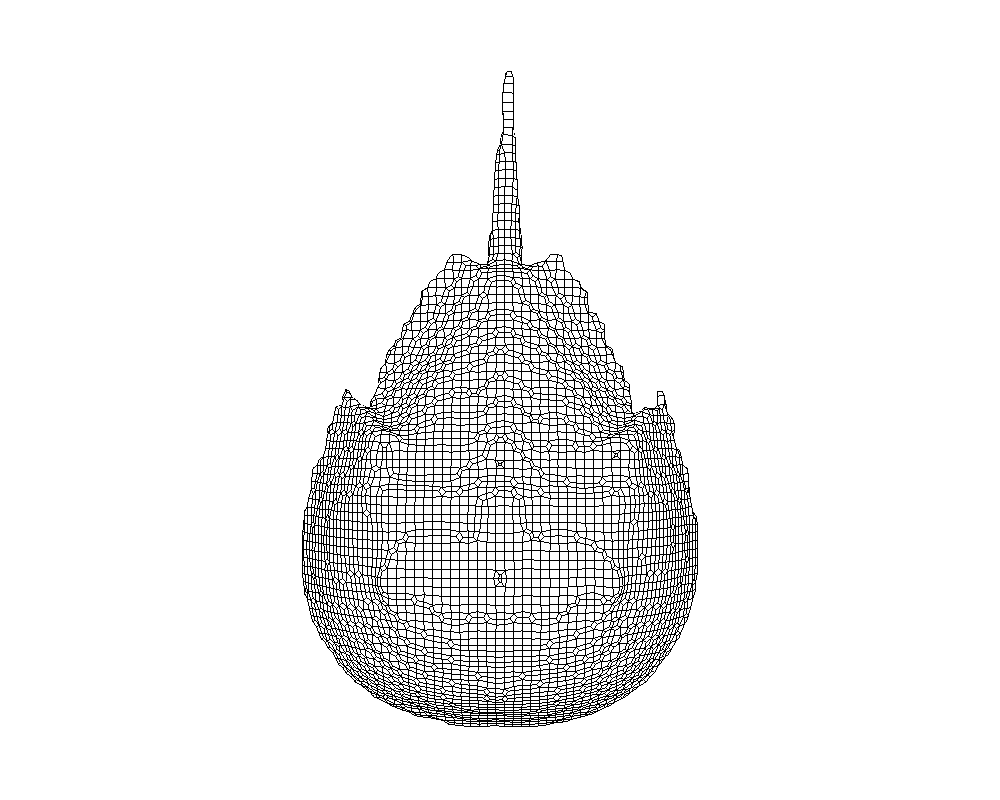
\includegraphics[width=0.45\textwidth]{ch22-crab-mesh-top.png}\\
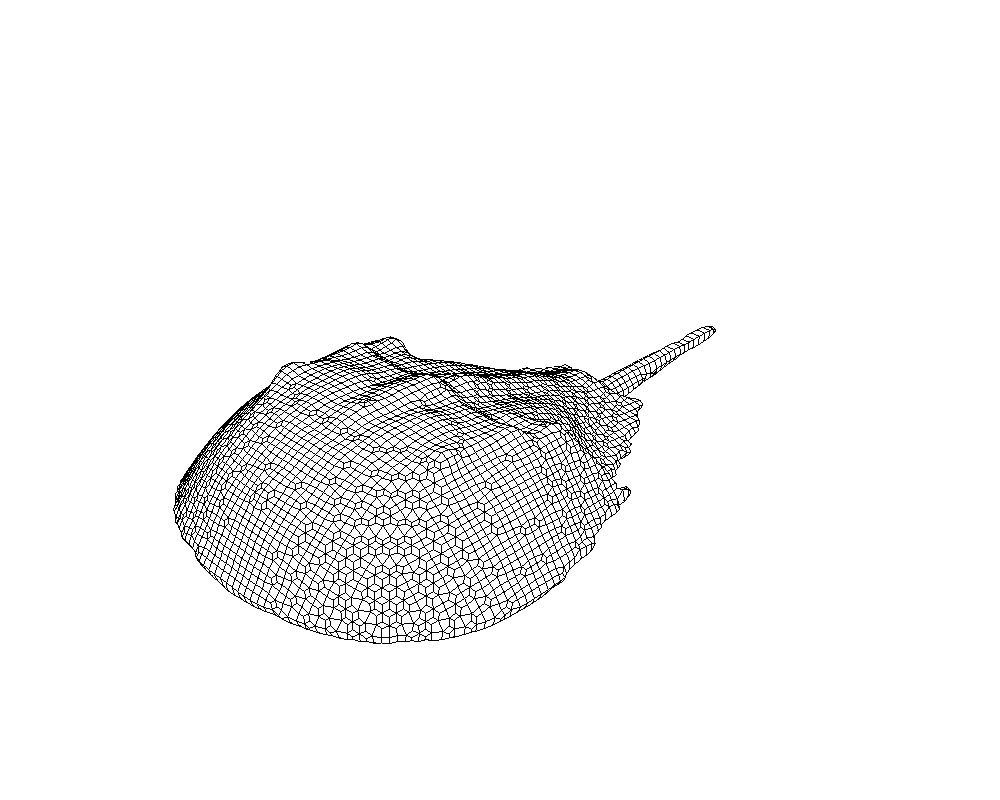
\includegraphics[width=0.72\textwidth]{ch22-crab-mesh.png}\\
\scriptsize The crab mesh from above and from the side (VisIt, the \code{.e} file as shipped).
\end{columns}
\end{frame}

% 22b
\begin{frame}{The horseshoe crab (2): the numbers}
\label{fr:crab2}
\scriptsize
\begin{tabular}{@{}L{0.14\textwidth}L{0.8\textwidth}@{}}
\toprule
tank & $L = 160$: $-80 < x < 80$, $-80 < y < 240$, $-80 < z < 80$ mm; the stream along $+y$; \code{domain\_boxes = [(0,0,0),(N - 1,2*N - 1,N - 1)]} \\
grid & three levels at ratio $4$, $N = 16$: $\mathrm{DX} = 160/256 = 0.625$ mm; about $20$ cells across the crab's thickness, $55$ across its width \\
stream & $V\,\dfrac{\tanh((t - t_{1/2})/\tau) + \tanh(t_{1/2}/\tau)}{1 + \tanh(t_{1/2}/\tau)}$ on all six faces, $V = 130$ mm/s, $t_{1/2} = 0.05$ s, $\tau = 0.125$ s: zero at $t = 0$, $V$ by $t \approx 0.4$ s (\code{VelocityBcCoefs\_1}) \\
Reynolds & $\rho V W/\mu \approx 4400$ with the width $W = 34$ mm; the input's \code{Re = 400.0} is written but not used (\code{MU} is set directly) \\
tether & the whole body: \code{kappa = kappa\_s} for every point (the test \code{if(s(0)<.2)} is commented out), \code{KAPPA\_S = 1e5} \\
material & $E = 700$ (stem) and $1400$ (leaf) Pa, $\nu = 0.3$, the same formulas as the plate; the leaf values are read and never used \\
time & \code{DT = 2e-5}, \code{END\_TIME = 1.0}: $50000$ steps; frames every $0.02$ s ($50$), restarts every $0.05$ s, data every $0.001$ s ($1000$ lines) \\
job & \code{script.sh}: $2$ nodes $\times$ $32$ tasks $= 64$ cores, $72$ hours, on a UNC cluster \\
\bottomrule
\end{tabular}

\medskip
\begin{itemize}
  \item $\mathrm{DT} = 2\times10^{-5}$ s with $\mathrm{DX} = 0.625$ mm and $V = 130$ mm/s is a CFL of $0.004$; the tether's $\kappa_s = 10^5$ g/(mm$^3$\,s$^2$) on a body of density $0.001$ is what sets it (chapter 19, slide 26).
  \item The stream along $+y$ and a tank twice as long in $y$: the crab sits $57$ mm from the inflow face and $207$ mm from the outflow, with its wake room to develop. The 2017 plate's one unit from the inflow was the lesson (slide \ref{fr:mapping3}).
\end{itemize}
\end{frame}

% 23
\begin{frame}[fragile]{The horseshoe crab (3): what the code measures}
\label{fr:crab3}
\footnotesize
\begin{columns}[T]
\column{0.5\textwidth}
\begin{lstlisting}[style=cpptiny]
static ofstream forcex_stream, forcey_stream, forcez_stream, velx_stream, ...,
                workx_stream, ..., U_L1_norm_stream, U_L2_norm_stream, U_max_norm_stream;
...   // in output_data, for each element and quadrature point:
F_integral[d] += F_node[k][d] * phi[k][qp] * JxW[qp];
U_integral[d] += U_node[k][d] * phi[k][qp] * JxW[qp];
W_integral[d] += U_node[k][d]*F_node[k][d] * phi[k][qp] * JxW[qp];
...
forcex_stream << loop_time << " " << F_integral[0] << endl;   // F_x.curve
velx_stream   << loop_time << " " << U_integral[0] << endl;   // U_x.curve
workx_stream  << loop_time << " " << W_integral[0] << endl;   // W_x.curve
\end{lstlisting}
\column{0.48\textwidth}
\begin{itemize}
  \item Twelve \code{.curve} files (VisIt's curve format: a time and a value per line, chapter 29): the force on the body integrated from the \code{F} system (stress plus tether: the total force the body puts on the fluid), the integral of the body's velocity (zero for a body that is held, a check), and $\int U_d F_d$ per component, whose sum over $d$ is the power the body puts into the fluid.
  \item The $L^1$, $L^2$ and max norms of the fluid velocity over the hierarchy (\code{U\_L1.curve}, \code{U\_L2.curve}, \code{U\_max.curve}): a check that the stream has reached its speed and that nothing is blowing up.
  \item \code{F\_y.curve} is the drag along the stream; \code{F\_x} and \code{F\_z} the side force and the lift. A plot of \code{F\_y} against time with the stream's ramp gives the drag coefficient once the force is steady; chapter 11's recipe.
\end{itemize}
\end{columns}
\end{frame}

% 23b
\begin{frame}{The horseshoe crab (4): what is wrong with it, and what a port needs}
\label{fr:crab4}
\scriptsize
\begin{itemize}
  \item \al{\code{U\_integral} is never set to zero}: the initialisation loop runs twice for \code{F\_integral} and never for \code{U\_integral}, so the \code{U\_*.curve} files hold whatever was in memory plus the integral. \code{W\_integral} is initialised. The fix is one line.
  \item \al{Leftovers:} \code{mu\_leaf}, \code{beta\_leaf}, \code{E\_LEAF} and \code{t\_set} are read and unused; the material test is commented out; \code{coordinate\_mapping\_function} (\code{X(0) = s(0)}) is defined and never registered; \code{MESH\_FILENAME} defaults to \code{"Leaf.e"}, a file from another project; \code{Re} is unused; every input line ends in \code{//} (the CRLF trick of slide \ref{fr:wrong}).
  \item \al{Old API:} \code{libMeshEnums::Order}, \code{SAMRAI\_MPI}, \code{AutoPtr}, \code{IBAMR\_config.h}: chapter 17's list applies before it compiles against 0.16.0 or later; \code{output\_data} then needs \code{IBTK\_MPI} and the current \code{FEBase::build} as in IBFE/10.
  \item \al{Cost:} $50000$ steps of a $256^3$-equivalent tank with a $21710$-element body on $64$ cores for up to $72$ hours. It has not been run for this series (IBFE/11 is pending); size it with a short run first, and expect the restart files to matter.
  \item \al{Angle of attack.} ``$0$deg'' in the zip's name; other angles come from the coordinate mapping (a rotation of \code{s}, slide \ref{fr:mapping2}) with the tether target rotated the same way, not from new meshes.
  \item \al{What the port would ship:} the mesh, a cleaned \code{main.cpp} with one \code{output\_data} that writes a single text file (time, three forces, three powers) as IBFE/10 does, an input with the ramp and the tank as above, a Puma job script sized from a timing run, and a README with the first hundred steps' force so that a run can be checked.
\end{itemize}
\end{frame}

% 24
\begin{frame}{Looking at a 3D run in VisIt}
\label{fr:visit}
\footnotesize
\begin{enumerate}
  \item Open \code{viz\_IB3d/dumps.visit}; \textbf{Add $\to$ Pseudocolor} with the expression \code{U[0]} (the $x$-velocity; \textbf{Controls $\to$ Expressions} to define it, or pick the component) and \textbf{Draw}: you see the outside of the box.
  \item \textbf{Operators $\to$ Slicing $\to$ Slice}: normal along $y$ ($0, 1, 0$) through the origin, the $x$--$z$ plane through the plate's middle. ``Project to 2D'' makes a flat picture with a 2D view; off, the slice stays in the box for a 3D camera.
  \item Open \code{viz\_IB3d/output.ex2}, \textbf{Add $\to$ Mesh}: the plate in its starting position. For the moving plate, the expression \code{dX = \{dX\_0, dX\_1, dX\_2\}} (three components now) and \textbf{Operators $\to$ Transforms $\to$ Displace} with it; a \textbf{Pseudocolor} of \code{dX\_0} on the plate shows the bend (slide \ref{fr:flaps}). To cut the plate with the same slice, add the Slice operator to its plot too: its cross-section appears on the 2D picture.
  \item The 3D camera: \textbf{View $\to$ 3D}, or drag; in a script, \code{View3DAttributes} with \code{viewNormal}, \code{focus}, \code{viewUp}, \code{parallelScale} (\code{wsl/final/visit\_ch22.sh}). A \textbf{Subset} plot of \code{levels} shows the grid levels (slide \ref{fr:levels}).
\end{enumerate}
\begin{itemize}
  \item \code{dumps.visit} has \code{U}, \code{P}, \code{Omega} (a vector), \code{Div U} and \code{F}; \code{output.ex2} has \code{dX\_*}, \code{X\_*}, \code{F\_*} and \code{U\_*} at the nodes. Chapter 27 is 3D visualization (isosurfaces, streamlines, clipping); chapter 28 the finite element data; chapter 30 movies.
  \item Chapter 21's ``Random info'' applies: open the fluid first, Draw, then the Exodus file.
\end{itemize}
\end{frame}

% 25
\begin{frame}{What can go wrong}
\label{fr:wrong}
\scriptsize
\renewcommand{\arraystretch}{0.92}
\begin{tabular}{@{}L{0.40\textwidth}L{0.52\textwidth}@{}}
\toprule
symptom & cause and fix \\
\midrule
\code{Illegal character token in input} at line 2 & the input file has Windows line endings; the course's fix was \code{//} at the end of every line, the clean one \code{dos2unix} (chapter 16) \\
libMesh cannot read the \code{.msh}, or reads nothing & gmsh 4 wrote MSH 4.1 binary or a file without physical groups; save as Version 2 ASCII with a physical volume (slide \ref{fr:gmsh3}, chapter 18) \\
``1D or 2D elements'' errors from libMesh & lines and surfaces saved along with the volume; define the physical volume so only it is saved, or \code{Mesh.SaveAll = 0} \\
the plate sits at the file's position although a mapping was registered & the mapping was registered after \code{initializeFEEquationSystems()}, or the tether pulls it back to \code{s} (slide \ref{fr:mapping2}) \\
the plate near the inflow face does nothing to the flow & it is inside the face's prescribed velocity (the 2017 $-7$); keep bodies away from prescribed faces (slide \ref{fr:mapping3}) \\
\code{J from -0.3 to ...}, then NaN & $J < 0$ in a sliver element and $\ln J$ undefined; reduce \code{DT}, optimise the mesh, lower $\kappa_s$ \\
``Max Jacobian 1 / Min Jacobian 1'' every step & the course code printed variables nothing updated; IBFE/10 records the real range \\
the run writes nothing for minutes & 3D is slow: $0.6$ s per step here; check the log for \code{At end of timestep} and the first \code{visit\_dump} \\
\code{U\_x.curve} full of garbage & the crab's uninitialised \code{U\_integral} (slide \ref{fr:crab4}) \\
\code{MFAC} changed, nothing happens & it does not apply to a mesh read from a file \\
the wake hits the outflow face & the outflow velocity is prescribed; lengthen the tank or use a traction condition (chapter 7) \\
\bottomrule
\end{tabular}
\end{frame}

% 26
\begin{frame}{What the older decks had that is now Part X}
\label{fr:legacy}
\footnotesize
\begin{tabular}{@{}L{0.46\textwidth}L{0.46\textwidth}@{}}
\toprule
2017--2020 & now \\
\midrule
the tank ``$-16 < x < 16$'' and the plate shifted by $-7$ & the input was already $-8 < x < 24$; \code{TRANSLATE\_X} as an option, tested (slide \ref{fr:mapping3}) \\
``middle half'' with \code{abs(s(2)) < .25} & \code{TWO\_MATERIALS} with \code{STEM\_HALF\_WIDTH} (slide \ref{fr:twomat}) \\
\code{vector<NumericVector<double>*>\& system\_data} (2017) & \code{var\_data} and \code{grad\_var\_data} (chapter 19) \\
\code{AutoPtr}, \code{libMeshEnums::Order}, \code{SAMRAI\_MPI}, \code{IBAMR\_config.h}, \code{abs} & \code{std::unique\_ptr}, \code{libMesh::Order}, \code{IBTK\_MPI}, no config headers, \code{std::abs} (chapter 17) \\
``Void PK1\_dil\_stress\_function'' (the 2020 slide 16 typo) & \code{void} \\
\code{data\_dump\_interval = 1} and an empty \code{output\_data} & $100$ tether-force lines per run \\
Makefile with \code{LIBSNEW} & \code{CMakeLists.txt} \\
\code{//} at the end of every input line & LF line endings \\
gmsh ``Add $\to$ Translate $\to$ Extrude'', ``group\_name.msh'' & Translate $\to$ Extrude; the file is named by you (slides \ref{fr:gmsh2}--\ref{fr:gmsh3}) \\
the horseshoe crab without slides & slides \ref{fr:crab}--\ref{fr:crab4}; the port is IBFE/11, pending \\
\bottomrule
\end{tabular}
\end{frame}

% 27
\begin{frame}{Exercises}
\label{fr:exercises}
\footnotesize
\begin{enumerate}
  \item Continue IBFE/10 to the course's $t = 2$ from its restart files (\code{END\_TIME = 2.0}, \code{restart\_IB3d 5000}). Plot $F_x(t)$ from \code{tether\_force.txt}: when does it stop changing, and what is the steady drag? Compare it with $\rho U^2 D^2 C_D/2$ for a plate at $\mathrm{Re} = 20$.
  \item Start the stream impulsively (\code{gcoef = "U0"}) and compare the first ten force lines with the $\tanh$ start's.
  \item \code{TRANSLATE\_X = 4.0}: check in VisIt that the plate sits at $x = 4$ and that \code{dX\_0} reads about $4$ there; then \code{TRANSLATE\_X = -7.0} and watch what the inflow face does to the force.
  \item \code{TWO\_MATERIALS = TRUE} to $t = 0.5$: how much more do the softer flaps bend? Then fix the $E$ swap and run again.
  \item \code{TETHER\_HALF\_WIDTH = 0.5}, the ``middle half'' the 2017 goal said: does the force change, and does the top edge still move more than the bottom one?
  \item \textbf{Mesh $\to$ Optimize 3D} on \code{plate2.msh} in gmsh (or extrude in three layers), run to $t = 0.1$, and compare the range of $J$ with the shipped mesh's $0.66$--$2.51$.
  \item \code{Re = 400} (\code{MU} four times smaller) with \code{DT = 5e-5}: does a wake leave the fine level's box? Add a threshold or widen the box.
  \item Initialise \code{U\_integral} in the crab's \code{output\_data}, remove the leftovers, and estimate from one hundred steps on four cores what the full run would cost.
\end{enumerate}
\end{frame}

% 28
\begin{frame}{Rules of thumb}
\label{fr:thumb}
\small
\begin{itemize}
  \item Six faces, the stream on all of them, nothing periodic; the body several kernel widths from any prescribed face, and its wake room to recover before the outflow.
  \item Volume elements about $\mathrm{DX}$ across, two or three through a thin body; a physical volume; MSH 2.2 ASCII; look for slivers before you run.
  \item The coordinate mapping places a body; whatever compares \code{X} with \code{s} must apply the same mapping.
  \item Time a short run first: $0.6$ s per step here on four cores; the course's $2$ time units are an afternoon.
  \item Minus the tether force is the force of the fluid on a held body; an accelerating stream pushes before it flows.
  \item $J$ far from $1$ in a few elements is a mesh defect; $J < 0$ is a run that will end.
  \item Slice, displace, then camera; the vorticity is a vector in 3D.
\end{itemize}
\end{frame}

% 29
\begin{frame}{Summary}
\label{fr:summary}
\footnotesize
\begin{enumerate}
  \item IBFE/10 puts a $2\times2\times0.125$ plate across a stream in a $32\times16\times16$ tank on three grid levels, holds its middle band with a tether, and lets the flaps bend; the stream is prescribed on all six faces and starts as $\tanh 2t$.
  \item The plate's mesh is a gmsh extrusion saved as a physical volume in MSH 2.2; its sliver tetrahedra are where $J$ strays and a few nodes jump.
  \item The initial coordinate mapping places the file's mesh in the tank before the first step; \code{s} stays the file's coordinates, so tethers and prescribed motions must be mapped too. It works in 0.19.0; the 2017 version's trouble was a plate one unit from the inflow face.
  \item A 3D run costs $0.6$ s per step on four cores and $100$ MB per $20$ frames; time it, write restarts, and keep the fine level to the body.
  \item The tether force, integrated over the plate at Gauss points, is minus the force of the fluid: $0.28$ at $t = 0.5$, with the acceleration of the stream in it; 0.16.0 and 0.19.0 agree to six digits.
  \item The horseshoe-crab example holds a $25864$-node body rigid in a $13$ cm/s stream at $\mathrm{Re} \approx 4400$ for $72$ hours on $64$ cores; its velocity integral is uninitialised and its API is the 2018 one; it is written up here for the first time and ported next.
\end{enumerate}
\begin{homebox}
\footnotesize Chapter 23 walks through a whole IBFE main file, line by line, with IBAMR's \code{ex7}.
\end{homebox}
\end{frame}

% 30
\begin{frame}{Recordings (listed, not incorporated)}
\label{fr:videos}
\small The 2020 Zoom recording of the IBFE lecture \emph{3D Flow Past Objects} and the 2018 Dogwood session that introduced the flow-tank and free-flow set-ups are listed in the front matter's video list (chapter 0.1). The 2020 deck's render is reproduced on slide \ref{fr:flow2}; the gmsh screenshots on slides \ref{fr:gmsh1}--\ref{fr:gmsh3}.
\end{frame}

% 31
\begin{frame}{References and credits}
\label{fr:refs}
\scriptsize
\begin{itemize}
  \item Example IBFE/10 of this series (\code{main.cpp}, \code{input3d}, \code{plate2.msh}, \code{job.slurm}, README with the measured tables); the runs \code{ft\_default}, \code{ft\_translate}, \code{ft\_twomat} with IBAMR 0.19.0 and \code{ft\_default} with 0.16.0; \code{wsl/final/visit\_ch22.sh}. Figures: VisIt 3.5.
  \item The course material: \emph{7-IBFE 3D Flow Tank} (Feb 2017, edited 2018) and its zip \code{Example\_IBFE\_FlowTank3d-mid\_plate} (2017); \emph{3-IBFE 3D Flow Past Objects} (2020) and its git history; the Dogwood deck (2018--20, private; numbers only); \code{examples/legacy/UA-Examples/IBFE Examples/3-IBFE-Example\_FlowTank-MidPlate} and \code{3-IBFE-Example-HorseshoeCrab} (course repository). The gmsh screenshots and the render are the 2020 deck's.
  \item IBAMR 0.19.0: \code{src/IB/IBFEMethod.cpp} (\code{getFromInput}: the \code{IB\_*}, \code{interp\_*} and \code{spread\_*} keys), \code{examples/IBFE/explicit/ex4} (compressible neo-Hookean, 2D and 3D) and \code{ex5} (a body held by penalty springs, with drag output). \url{https://github.com/IBAMR/IBAMR}
  \item gmsh: C. Geuzaine and J.-F. Remacle, \emph{Gmsh: a three-dimensional finite element mesh generator with built-in pre- and post-processing facilities}, Int.\ J.\ Numer.\ Meth.\ Engng 79 (2009) 1309--1331. \url{https://gmsh.info}
\end{itemize}
\end{frame}

\end{document}
